%        File: covo.tex
%     Created: Di Okt 16 10:00  2018 C
% Last Change: Di Okt 16 10:00  2018 C
%

\documentclass[a4paper]{report}
% ***************************PACKAGES***************************
\usepackage{graphicx}
\usepackage{caption,setspace}
\usepackage{subcaption}
\captionsetup[figure]{width=0.7\textwidth,font={small}}
\usepackage{float}
\usepackage{amsmath}
\usepackage{amssymb}
\usepackage{hyperref}
\usepackage{siunitx}
\usepackage{graphicx}
\usepackage{subcaption}
\usepackage{mwe}
\usepackage{tabularx}
\usepackage{cite}
\usepackage{hyperref}
\usepackage{bookmark}
\usepackage{algorithm}
\usepackage[noend]{algpseudocode}
\usepackage{array}


% ***************************CONFIGS***************************
% for numbering per section
\numberwithin{figure}{section}
% removing ugly colored rectangles from references
\usepackage{xcolor}
\hypersetup{
    hidelinks,
    colorlinks = false,
    %linkcolor={black},
    %citecolor={black},
    %urlcolor={black}
  }
% command for table tabular alignment
\newcolumntype{L}{>{\raggedright\arraybackslash}X}
% command for argmin and argmax
%\DeclareMathOperator*{\argmax}{arg\,max}
%\DeclareMathOperator*{\argmin}{arg\,min}
\newcommand{\argmin}{\mathop{\mathrm{argmin}}}
\newcommand{\argmax}{\mathop{\mathrm{argmax}}}
\newcommand{\R}{\mathbb{R}}
% commands for cascading subfigures
\newsavebox{\subfloatbox}
\newcommand{\topfloat}[2][\empty]% #1 = caption, #2=image
 {\savebox\subfloatbox{#2}%
  \begin{minipage}[t]{\wd\subfloatbox}
    \usebox\subfloatbox
    \subcaption{#1}
  \end{minipage}}
\newcommand{\bottomfloat}[2][\empty]% #1 = caption, #2=image
 {\savebox\subfloatbox{#2}%
  \begin{minipage}[b]{\wd\subfloatbox}
    \captionsetup{position=top}%
    \subcaption{#1}
    \usebox\subfloatbox
  \end{minipage}}

\algnewcommand\algorithmicforeach{\textbf{for each}}
\algdef{S}[FOR]{ForEach}[1]{\algorithmicforeach\ #1\ \algorithmicdo}

\newcommand*{\vertbar}{\rule[-1ex]{0.5pt}{2.5ex}}
\newcommand*{\horzbar}{\rule[.5ex]{2.5ex}{0.5pt}}


% ***************************ACRONYMS***************************
\usepackage[toc, shortcuts]{glossaries}
\makeglossaries
\newacronym{vo}{VO}{Visual Odometry}



\begin{document}

% ***************************TITLE***************************
\begin{titlepage}
\begin{center}

%  
\includegraphics[width=\textwidth]{../fig/tuc_logo.jpg}

\vspace{1.5cm}


{\Huge \textbf{Master Thesis}}\\
\vspace{0.5cm}
{\huge \textbf{An Error Aware RGB-D \\Visual Odometry}}


\vspace{2.5cm}

{\huge \textbf{U\u{g}ur Bolat}}

\vfill

Date:

\vspace{1.2cm}

Supervisors: \\
Dr.-Ing. Sven Lange \\
M.Sc. Tim Pfeifer

\vspace{0.8cm}

Faculty of Electrical Engineering and Information Technology\\
Professorship of Process Automation

\end{center}
\end{titlepage}

% ***************************TABLE OF CONTENT ETC.***************************
\tableofcontents
\newpage
\listoffigures
\listoftables
\newpage
\printglossary[type=\acronymtype,title={Abbreviations}]
\newpage

% ***************************DOCUMENT***************************

\begin{abstract}


\end{abstract}

\newpage

% ***************************CP1-INTRO***************************
\chapter{Introduction} \label{cp_intro}


\newpage

% ***************************CP2-VO***************************

\chapter{Camera Models} \label{cp_cam_models}

A camera maps from a 3D world scene to a 2D image plane. We call this process 
projection operation. Since the \acrshort{vo} systems process camera image 
sequences, one has to model this projection operation accurately. One of the 
basic camera modeling technique is the \textit{Pinhole Model} where the projection of 
the 3D points are mapped on a 2D image plane (also called focal plane). 

\section{The Pinhole Model} \label{sbsc_pinhole}

In this model, the camera centre sits behind the image plane.
The Z-axis, 
also called \textit{principal axis}, of this 
coordinate system points out through the origin of the image plane and the 
point where pierce through image plane is called the \textit{pricipal point}. 
We can also see how other two axes are located in Figure-\ref{fig:pinhole} 
and this is known as the \textit{Camera Coordinate System} $(x_{cam}, y_{cam}, z_{cam})$.


\begin{figure}[H]
	\centering
	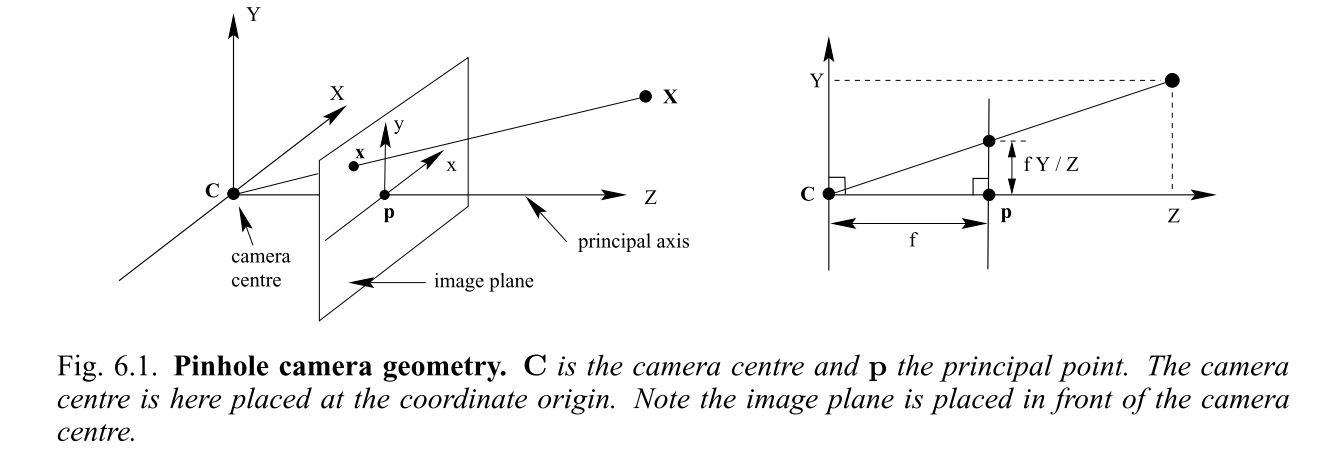
\includegraphics[width=\linewidth,natwidth=640,natheight=640]
  {fig/ref_imgs/pinhole_model.png}
  \caption{REMEMBER TO DRAW HORIZ/VERT Fx and Fy. The Pinhole Model}
	\label{fig:pinhole}
\end{figure}

Thanks to geometrical propotion property, we can project 
the 3D point $(X, Y, Z)^T$ in Euclidean space $\mathbb{R}^3$
to the 2D point $(U,V)^T = (f_xX/Z, f_yY/Z)^T$ in Euclidean space $\mathbb{R}^2$, 
where $f_x$ and $f_y$ are the \textit{focal lengths} 
between the camera centre and the pricipal 
point with respect to horizontal and vertical axis of the Camera Coordinate 
System respectively.
After projection, we obtain a 2D 
point that we represent on the 
\textit{Image Coordinate Frame} $(u_{img},v_{img})$.

To be more specific,
we can write the projection operation as a linear mapping function 
in the following way if we utilize the homogenous coordinates:

NOTE: NAME x,y,z indices for world and camera coords all below

\begin{equation}
  \begin{pmatrix}
    U\\
    V\\
    1
  \end{pmatrix}
  \sim
  Z
  \begin{pmatrix}
    f_xX/Z\\
    f_yY/Z\\
    1
  \end{pmatrix}
  =
  \begin{pmatrix}
    f_xX\\
    f_yY\\
    Z
  \end{pmatrix}
  =
  \begin{bmatrix}
    f_x & 0 & 0 & 0\\
    0 & f_y & 0 & 0\\
    0 & 0 & 1 & 0\\
  \end{bmatrix}
  \begin{pmatrix}
    X\\
    Y\\
    Z\\
    1
  \end{pmatrix}
\end{equation} \label{eq:proj_func_w_f}

This equation applies for the case when 3D points are 
projected onto a plane where the principal point is the origin. 
However, the common convention in partice 
is to have the origin at the (not entirely sure) left-bottom corner not in the centre.

\begin{figure}[H]
	\centering
	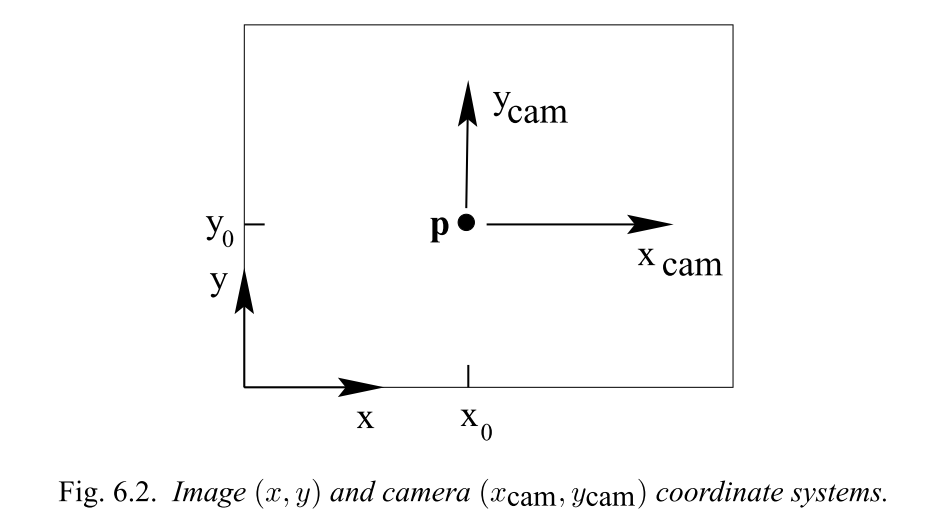
\includegraphics[width=\linewidth,natwidth=640,natheight=640]
  {fig/ref_imgs/pinhole_offset.png}
	\caption{Principle Point Offset}
	\label{fig:pinhole_offset}
\end{figure}

Thus, we get offsets, which can further be added into our function:

\begin{equation}
  \begin{pmatrix}
    U\\
    V\\
    1
  \end{pmatrix}
  \sim
  Z
  \begin{pmatrix}
    (f_xX + Z c_x)/Z\\
    (f_yY + Z c_y)/Z\\
    1
  \end{pmatrix}
  =
  \begin{pmatrix}
    f_xX + Z c_x\\
    f_yY + Z c_y\\
    Z
  \end{pmatrix}
  =
  \begin{bmatrix}
    f_x & 0 & c_x & 0\\
    0 & f_y & c_y & 0\\
    0 & 0 & 1 & 0\\
  \end{bmatrix}
  \begin{pmatrix}
    X\\
    Y\\
    Z\\
    1
  \end{pmatrix}
\end{equation} \label{eq:proj_func_w_f_c}

where $c_x$ and $c_y$ are coordinates of the principal point \textbf{p}.

In addition to pricipal offsets, inaccurately synchronized pixel-sampling 
process can result in \textit{skewed pixels}. This camera imperfection leads to 
non-square pixels as seen in Figure-\ref{fig:skewed}.

\begin{figure}[H]
	\centering
  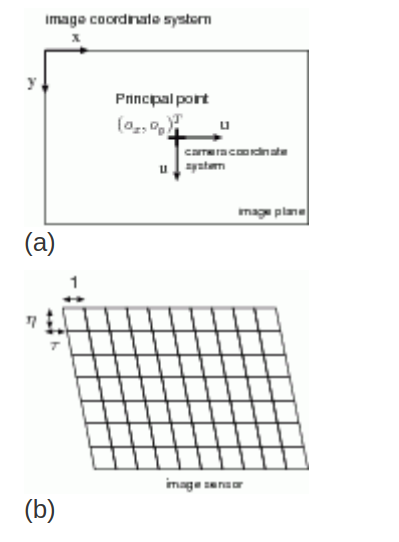
\includegraphics[width=0.5\linewidth,natwidth=640,natheight=640]
  {fig/ref_imgs/skew.png}
  \caption{REMEMBER TO DRAW FOR X and Y.Skew and Non-Square Pixels}
	\label{fig:skewed}
\end{figure}

We can scale the square pixels, having 1:1 pixel aspect ratio, with the 
corresponding skew parameters $\eta_x$, $\eta_y$ and $s$:

\begin{equation}
  \begin{pmatrix}
    U\\
    V\\
    1
  \end{pmatrix}
  \sim
  \begin{bmatrix}
    f_x\eta_x & s & c_x & 0\\
    0 & f_y\eta_y & c_y & 0\\
    0 & 0 & 1 & 0\\
  \end{bmatrix}
  \begin{pmatrix}
    X\\
    Y\\
    Z\\
    1
  \end{pmatrix}
  =
  \begin{bmatrix}
    \alpha_x & s & c_x & 0\\
    0 & \alpha_y & c_y & 0\\
    0 & 0 & 1 & 0\\
  \end{bmatrix}
  \begin{pmatrix}
    X\\
    Y\\
    Z\\
    1
  \end{pmatrix}
\end{equation} \label{eq:proj_func_w_square_pix_skew}

Generally, the skewed pixels issues occurred in ealier versions of CCD cameras 
and this is mostly fixed in new generation digital cameras. Therefore, 
we can neglate this effect by taking $\eta_x=1$, $\eta_y=1$ and $s=0$.

Next, we can extract:

\begin{equation}
  \mathbf{K} = 
  \begin{bmatrix}
    \alpha_x & s & c_x\\
    0 & \alpha_y & c_y\\
    0 & 0 & 1\\
  \end{bmatrix}
\end{equation} \label{eq:k_matrix}

The $\mathbf{K}$ matrix is called 
\textit{intrinsic parameters matrix}, which represents the characteristics of 
a camera sensor. Note that, we 
can further reformulate the notation \ref{eq:proj_func_w_square_pix_skew} in more 
compact form:

\begin{equation}
  \mathbf{x_{img}} = \mathbf{K}[\mathbf{I}|\mathbf{0}]\mathbf{X_{cam}}
\end{equation} \label{eq:simplyfied_proj_func}

\begin{figure}[H]
	\centering
  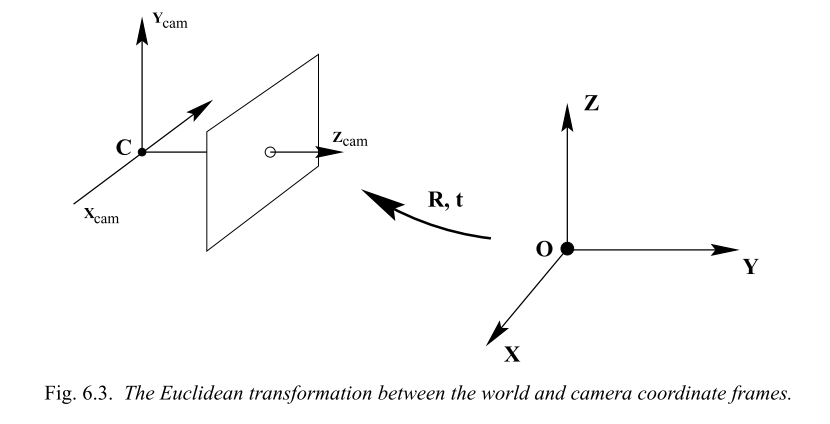
\includegraphics[width=\linewidth,natwidth=640,natheight=640]
  {fig/ref_imgs/cam_model_rot_trans.png}
  \caption{Camera Rotation and Translation}
  \label{fig:cam_model_rot_trans}
\end{figure}

Remember that, the Z-axis of the Camera Coordinate System aligns with the 
principal axis that is \textit{local} to camera frame. In fact, we have 3D points that 
we represent in the \textit{World Coordinate System} 
which we refer as the \textit{global} frame. 
These two coordinates systems 
can be transformed one another by a rotation and a translation as it is 
depicted in Figure-\ref{fig:cam_model_rot_trans} but we are interested in 
converting from the World Coordinate to Camera Coordinate System in this case.
To do so, we first perform series of rotations around each axis of the 
cartesian coordinate system in Euclidean space by using 
\textit{rotation matrices} where $R_x, R_y, R_z \in SO(3)$ is the rotation group:

\begin{equation}
  R_x(\theta) = 
  \begin{bmatrix}
    1 & 0 & 0\\
    0 & cos\theta & -sin\theta\\
    0 & sin\theta & cos\theta
  \end{bmatrix}
\end{equation} \label{eq:rot_matrx_x}

\begin{equation}
  R_y(\theta) = 
  \begin{bmatrix}
    cos\theta & 0 & -sin\theta\\
    0 & 1 & 0\\
    sin\theta & 0 & cos\theta
  \end{bmatrix}
\end{equation} \label{eq:rot_matrx_y}

\begin{equation}
  R_z(\theta) = 
  \begin{bmatrix}
    cos\theta & -sin\theta & 0\\
    sin\theta & cos\theta & 0\\
    0 & 0 & 1
  \end{bmatrix}
\end{equation} \label{eq:rot_matrx_z}

One can concatenate all three rotations about axes z, y, x respectively:

\begin{equation}
  \mathbf{R} = \mathbf{R_z(\gamma)}\mathbf{R_y(\beta)}\mathbf{R_x(\alpha)}
  =
  \begin{bmatrix}
    r_{11} & r_{12} & r_{13}\\
    r_{21} & r_{22} & r_{23}\\
    r_{31} & r_{32} & r_{33}\\
  \end{bmatrix}
\end{equation} \label{eq:rot_matrix_derivation}

Then, perform a translation $\mathbf{t} \in \R^{3x1}$:

\begin{equation}
  \mathbf{t} = 
  \begin{bmatrix}
    t_x \\ t_y \\ t_z
  \end{bmatrix}
\end{equation} \label{eq:translation}

We can also compound the rotation matrix and the translation vector into 
one matrix:

\begin{equation}
  \mathbf{T} =
  \begin{bmatrix}
    r_{11} & r_{12} & r_{13} & t_x\\
    r_{21} & r_{22} & r_{23} & t_y\\
    r_{31} & r_{32} & r_{33} & t_z\\
  \end{bmatrix}
\end{equation} \label{eq:transformation_matrix}

The $\mathbf{T} \in \R^{4x3}$ matrix in fact represents 
a \textit{rigid-body transformation}, which we call 
\textit{extrinsic camera parameters}.

Finally, we combine intrinsic $\mathbf{K}$ and 
extrinsic $\mathbf{T}$ matrices to form the following notation: 

\begin{equation}
  \mathbf{x_{img}} = 
  \mathbf{P}\mathbf{X_{world}} = 
  \mathbf{K}\mathbf{T}\mathbf{X_{world}} = 
  \mathbf{K}[\mathbf{R}|\mathbf{t}]\mathbf{X_{world}} =
  \mathbf{K}\mathbf{X_{cam}}
\end{equation} \label{eq:simplyfied_proj_func_1}

\begin{equation}
  \mathbf{x_{img}} = \mathbf{F_{proj}}(\mathbf{X_{world}})
\end{equation} \label{eq:simplyfied_proj_func_2}

where $\mathbf{F_{proj}}(\mathbf{X_{world}})$ is the 
\textit{projective transformation function}, which takes 
the 3D points in the World Coordinate System, transforms to 
the Camera Coordinate Systems and then maps them into the Image 
Coordinate Systems.

To build any reliable computer vision application with digital cameras, it is 
to important to find a good $\mathbf{P}$ \textit{projection matrix}. 
The next section describes one of many numerical methods for estimationg this 
matrix in literature.

\section{Camera Calibration} \label{sb_sc_calibration}


It is important to note that derivations of the formulation of this section
is not provided. Therefore, I refer readers to \cite{bla} for the detailed 
formulation. However, the intiution of the calibration process is fairly 
straightforward. 

\begin{figure}[H]
	\centering
  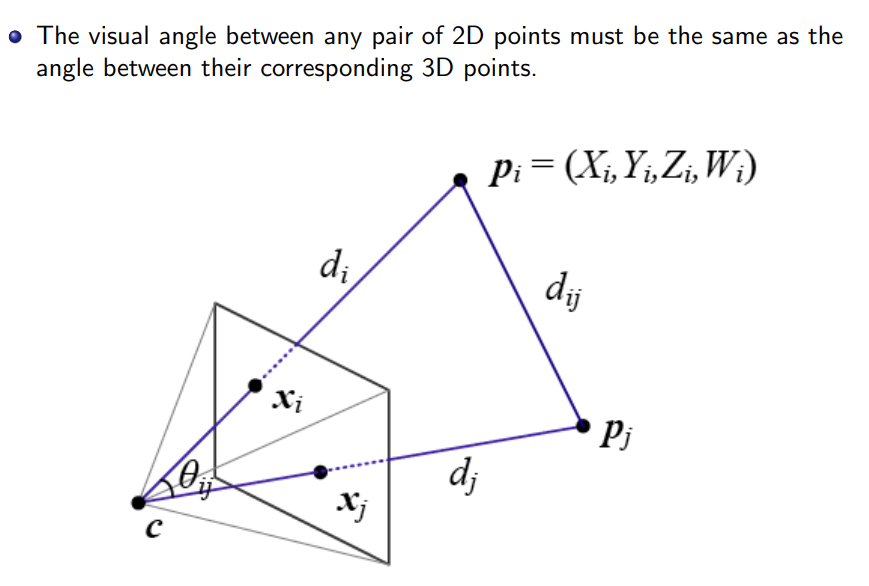
\includegraphics[width=\linewidth,natwidth=640,natheight=640]
  {fig/ref_imgs/calibration_dlt.png}
  \caption{Inheret Constraint}
  \label{fig:calibration_constraint}
\end{figure}


Assuming that we project two 3D points onto our image plane
like in Figure-\ref{fig:calibration_constraint},
the visual angle between those pair of 3D points is equal to 
the angle between its corresponding 2D points. This geometric constraints 
allow us to build the calibration problem. Remember that the goal is to find 
the projection matrix and we can build the problem in the following way:

\begin{equation}
  \mathbf{x_{img}} = 
  \begin{pmatrix}
    u_i\\
    v_i
  \end{pmatrix}
  =
  \mathbf{P}\mathbf{X_{world}} = 
  \begin{bmatrix}
    p_{00} & p_{01} & p_{02} & p_{03}\\
    p_{10} & p_{11} & p_{12} & p_{13}\\
    p_{20} & p_{21} & p_{22} & p_{23}
  \end{bmatrix}
  \begin{pmatrix}
    X_i\\
    Y_i\\
    Z_i\\
  \end{pmatrix}
\end{equation} \label{eq:proj_matrix}

Let's now distribute 
the projection matrix onto the 3D point measurement to retrieve individual 
pixel coordinates:

\begin{equation}
  u_i = 
  \frac
  {p_{00}X_i + p_{01}Y_i + p_{02}Z_i + p_{03}}
  {p_{20}X_i + p_{21}Y_i + p_{22}Z_i + p_{23}}
\end{equation} \label{eq:u_i}

\begin{equation}
  v_i = 
  \frac
  {p_{10}X_i + p_{11}Y_i + p_{12}Z_i + p_{13}}
  {p_{20}X_i + p_{21}Y_i + p_{22}Z_i + p_{23}}
\end{equation} \label{eq:v_i}


Since $\mathbf{x_{img}}$ and $\mathbf{X_{world}}$ are known,
we can find elements of the $\mathbf{p} = (p_{00}, p_{01}, \dots, p_{23})^T$ matrix 
by solving $\mathbf{Ap=0}$ liner system of equations from \ref{eq:u_i} and \ref{eq:v_i}.

For \textit{minimal solution} of this linear system of equations, 
we need at least $n \geq 6$ measurement points to solve the problem as 
the $\mathbf{P}$ matrix has 12 degree of freedom (11 if scale is ignored).
Note that this accounts for having 
noise-free measurement which does not hold in reality. Then, the problem 
becomes \textit{over-determined}.

In noisy measurement case, the problem is usually solved with
\textit{singular value decomposition (SVD)} with $n \geq 6$ measurement points. 
This method is called the \textit{Direct Linear Transformation (DLT)}.
Disadvantange of the DLT methods, it is still sensitive errors since 
it only considers \textit{algebraic errors}, which are the residuals of 
$\mathbf{Ap}$. 

While estimating the intrinsic and extrinsic parameters 
that are in linear form with the DLT, 
another issue known as \textit{radial distortion} 
has to take into account as well. This issue is caused by camera lens 
and Figure-\ref{fig:cam_distortion} depicts this effect and the straight lines 
appear to be curved. 

\begin{figure}[H]
	\centering
  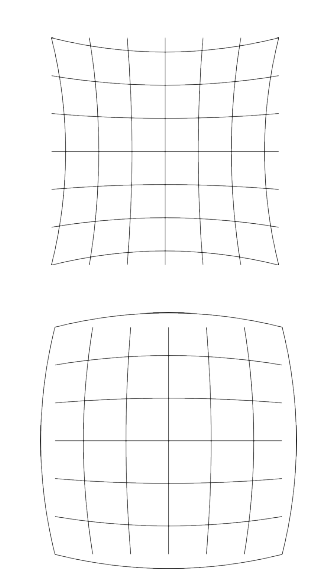
\includegraphics[width=0.3\linewidth,natwidth=640,natheight=640]
  {fig/ref_imgs/cam_distortion.png}
  \caption{Camera Distortion}
  \label{fig:cam_distortion}
\end{figure}

This distortion has non-linear characteristics and we also 
need to estimate the coefficients 
$\kappa = (k_1, k_2, p_1, p_2, k_3)^T$ of the following polynomial:


\begin{equation}
\begin{split}
  x''_i = F_{dist}(x') = 
  x'(1+ k_1 r^2 + k_2 r^4 + k_3 r^6) + 2 p_1 x' y' + p_2 (r^2+2x'^2)\\
  y''_i = F_{dist}(y') = 
  y'(1+ k_1 r^2 + k_2 r^4 + k_3 r^6) + p_1 (r^2+2y'^2) + 2p_2 x'y'\\
\end{split}
\end{equation}

where $x' = X_{cam}/Z_{cam}$ and $y' = Y_{cam}/Z_{cam}$. 
Note that, in \ref{eq:simplyfied_proj_func}, we first transform 
3D points from World Coordinate to Camera Coordinate Systems with 
extrinsic matrix and then we project them with the instrinsic matrix. 
To improve our pinhole camera model, 
we need to distort 3D points in the Camera Coordinate System before 
multiplying with the intrinsic matrix:

\begin{equation}
  \begin{pmatrix}
    U\\
    V\\
    1
  \end{pmatrix}
  =
  \begin{pmatrix}
    f_x x'' + c_x\\
    f_y x'' + c_y\\
    1
  \end{pmatrix}
    =
    F_{dis}\begin{pmatrix}
      \mathbf{K}
      \begin{pmatrix}
        X_{cam}\\
        Y_{cam}\\
        Z_{cam}\\
        1
      \end{pmatrix}
    \end{pmatrix} 
    =
    F_{dist}\begin{pmatrix}
      \mathbf{K} [\mathbf{R}|\mathbf{t}]
      \begin{pmatrix}
        X_{world}\\
        Y_{world}\\
        Z_{world}\\
        1
      \end{pmatrix}
    \end{pmatrix}
\end{equation} \label{eq:proj_func_w_f_c}

Above operations introduce non-linearity, which cannot be solved by DLT.
To get better accuracy at our projection matrix along with the distortion, 
\textit{least squares estimation}, i.e., Levenberg-Marquardt, is perfomed.

\begin{figure}[H]
	\centering
  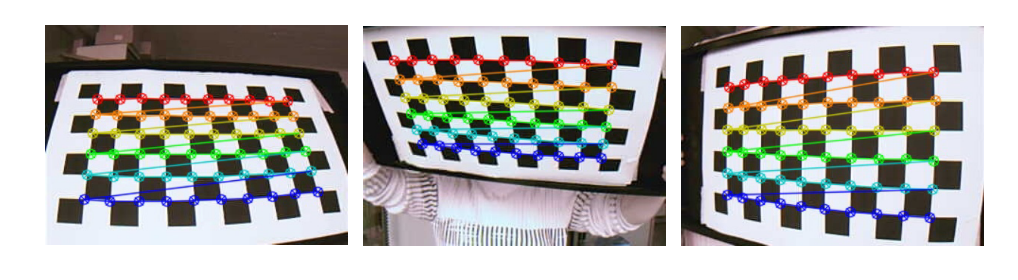
\includegraphics[width=\linewidth,natwidth=640,natheight=640]
  {fig/ref_imgs/checkerboard.png}
  \caption{Checkerboard}
  \label{fig:checkerboard}
\end{figure}

In practice, the checkerboard is used to get many good measurement points 
as  we easily extract edge features from the image. Now, the DLT comes handy
as we can use the DLT's result as an initial guess 
in the least squares optimization problem.

\begin{equation}
  \argmin_{\mathbf{p} \rightarrow \mathbf{K}, \kappa, \mathbf{R}_i, \mathbf{t}_i}
  \sum_{i=1:n} || \mathbf{x_{i}} - 
  \mathbf{P} \mathbf{X_{i}} ||^2
\end{equation}\label{eq:proj_lsq}

where $\mathbf{K}$ is the intrinsic matrix, 
$\kappa$ is the distortion coefficients, 
$\mathbf{R_i}$ is the corresponding orientation and 
$\mathbf{t_i}$ is the corresponding translation.
The afromentioned calibration process is well-studied problem in literature. 
Fortunately, there are many software libraries, such as OpenCV, 
that offers such implementations.



\chapter{Visual Odometry} \label{cp_vo}

\section{Image Features} \label{sc_img_features}

Image features are a collection of regions of interest or of points of interest 
that describe the image. In this way, we compress the necessary information 
from images so that we can achieve computationaly expensive task more efficiently.
Points of interest, also called \textit{keypoints}, 
are particularly valuable because their location in the image can be 
measured accurately. This is useful for localization related tasks such as VO. 

\subsection{Feature Extraction} \label{sb_sc_feature_extraction}

Generally, the goal is to find good features in feature-based VO. 
What defines a good feature is that it must be distinct, 
repeatable, computationaly cheap and invariant to geometrical changes. 
Obviously, one has many options to produce such image 
feautes but two common methods that are widely used in VO systems are 
blobs and corners. 
Blobs are image patterns that contain distinct image response comparing to their 
neighborhood pixels. Blobs take advantage of pixel intensity or color to 
decide whether it has a distinct response or not.
In the VO literature, SIFT\cite{}, SURF\cite{} or CENSURE\cite{} are popular 
choices for detecting blob featurus.
Corners are the meeting points where two or many edges intersect. Corners 
take advantage of geometrical structure of an image. FAST\cite{}, Shi-Tomasi or 
Haris\cite{} are widely used for detecting corners.

Fundemantally, a two-step process is needed to extract good features. 
First, you take a response function, called \textit{image filter}, 
shift this filter through the image and save the one that have greater 
response than your previously defined threshold as Keypoints.
In blob case, this might a Gaussian filter or a 
corner detector filter in corner case. Second, you perform non-maxima 
suppression on the resulting keypoints to find local minima of the function. 
The second step ensures you get keypoints only with maximum confidence. 

Inheritly, each feature detector has certain limitations and one has to 
choose whihc detector to use according to task objectives. Therefore, one can ask 
does the localization envorinment involve more texture oriented objects like 
floors, walls etc. or geometrical shapes like urban areas where many lines 
exist?
However, rule of thumb when choosing feature detector is that blobs 
are distinct but slow to compute and corners are fast to compute but less 
distict. 

\subsection{Feature Descriptor} \label{sb_sc_feature_descriptor}

Extracting features is the very first step of VO. The next step is to 
encode the detected keypoints into a format that we can perform comparison 
or search operation among them. This is done by taking the neighboring pixels 
around the keypoints and convert into a more compact form. For example, SIFT 
creates a patch around a keypoint, divides this patch into smaller grids,
calculate the gradient of each grid and 
saves into a histogram form.
This procedure makes feature descriptor 
robust agaist scale or rotation changes. Then, one can use these descriptors for 
various comparison operations such as matching or tracking in VO.


\subsection{ORB} \label{sb_sc_orb}

One of the most strict requirements of VO is the real-time contraints since it is 
expected to work at similari to low-sensors, i.e., accelerometer, gyroscopes etc. 
As previously discussed, blobs detectors are computationaly expensive. Therefore, 
corners based feature detector are more prevelant in VO. 
\textit{ORB (oriented FAST and rotated BRIEF)} studied known issues of 
FAST detector and BRIEF descriptor. Then, it fixed them into a level that 
it perform as accurate as SIFT, plus faster. Here are steps on how to extract features 
and create descriptors with ORB: 

\begin{enumerate}
  \item \textbf{Detect corners with FAST}: FAST take each pixel on 
    the image and compare with its adjacent pixels. More specificially, 
    ORB uses FAST-9, which takes a patch of discrete circular radius of $r=9$. 

    \begin{figure}[H]
	\centering
  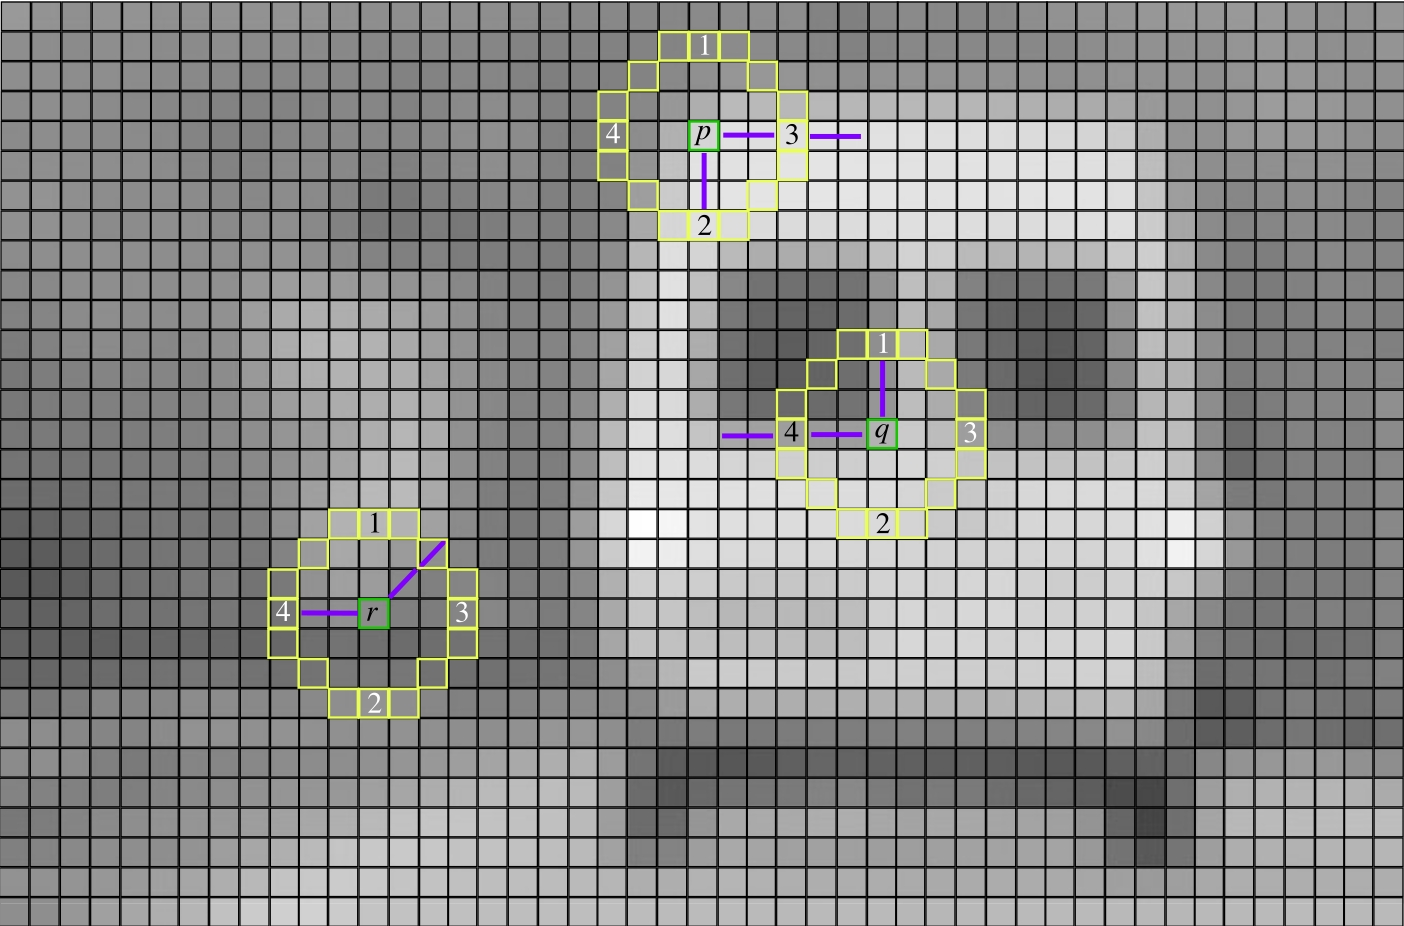
\includegraphics[width=0.6\linewidth,natwidth=640,natheight=640]
  {fig/ref_imgs/fast.png}
  \caption{FAST corners}
  \label{fig:fast_corners}
\end{figure}

    If the 
    selected pixel is $\pm t$ darker or brighter than adjacent pixels, 
    we call it a corner, where $t$ is our empiric threshold.

\begin{equation}
  M_c(p) = 
  \sum_{r \in S_{bright}} |I_{p \rightarrow r} - I_p| - t \text{ or } 
  M_c(p) = 
  \sum_{r \in S_{dark}} |I_p - I_{p \rightarrow r}| - t)
\end{equation}
    We retrieve $M^c_{1:n}$ the set of corner candidates from 
    comparing $I_{p\rightarrow x}$ the adjacent pixels around $I_p$ the target pixel.

  \item \textbf{Rank detected keypoint with Harris}: After FAST detection, 
    we get many corner candidates around the interest point. However, 
    FAST does not measure how good a corner is. Thus, we use Harris corner 
    detector to rank corner candidates:
    \begin{equation}
      \mathbf{A} = \sum_{x,y} w(x,y) 
      \begin{bmatrix}
        I_x^2 & I_xI_y \\ I_xI_y & I_y^2
      \end{bmatrix}
    \end{equation}
    The $\mathbf{A}$ matrix is calculated by the $I_x$ and $I_y$ partial 
    derivatives with respect to x and y direction and $w(x,y)$ weighting window.

    \begin{equation}
      R^c = det(\mathbf{A}) - k(trace(\mathbf{A}))^2
    \end{equation}
    where $det(\mathbf{A}) = \lambda_1 \lambda_2$ and 
    $trace(\mathbf{A}) = \lambda_1 + \lambda_2$.
    Then, we use the resulting $\mathbf{A}$ to find a ranking score for each 
    corner. Now, it is possible to take top N corners if desired.

  \item \textbf{Calculate orientation of corners with image moments}: 
    ORB uses BRIEF to create feature descriptors; however, BRIEF fails in 
    rotated images. Therefore, ORB modifies the BRIEF by adding orientation 
    information. To get orientation, an \textit{image moment} are calculated
    for each patch $S$:

    \begin{equation}
      m_{a,b}(S) = \sum_{x,y \in S} x^a y^b I(x,y)
    \end{equation}
    where $a + b$ defines the order of the moment and we need 
    the moments of order one:

    \begin{equation}
      m_{1,0}(S) = \sum_{x,y \in S} x \cdot I(x,y) \text{  ,  }
      m_{0,1}(S) = \sum_{x,y \in S} y \cdot I(x,y)
    \end{equation}

    Then, we get the orientation of the patch S:
    \begin{equation}
      \theta(S) = atan2(m_{01}, m_{10})
    \end{equation}

  \item \textbf{Form BRIEF descriptors with their corresponding orientation}:
    Once the top N corners and their orientations are detected, descriptions 
    can be formed with BRIEF. 

\begin{figure}[H]
	\centering
  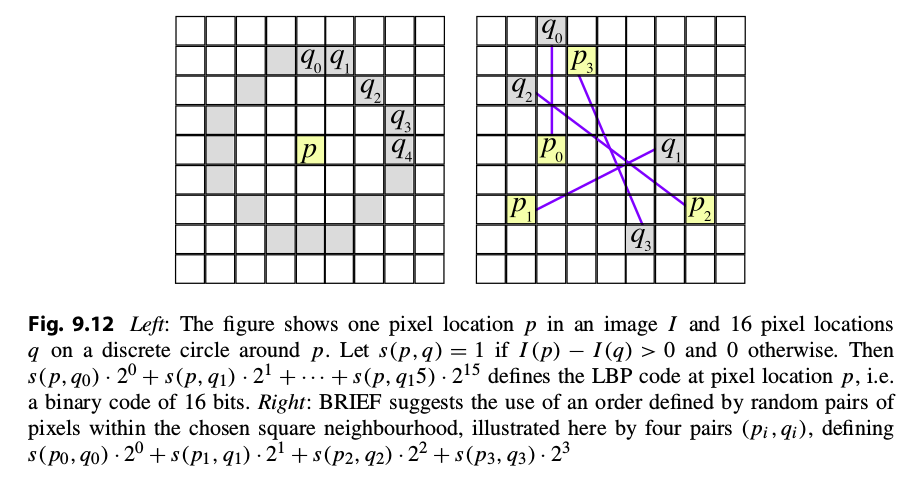
\includegraphics[width=\linewidth,natwidth=640,natheight=640]
  {fig/ref_imgs/brief.png}
  \caption{BRIEF pairs}
  \label{fig:brief_pairs}
\end{figure}


    To do so, we randomly (generated by normal distribution) 
    selected 256 pairs $(p_i,q_i)$ 
    inside the patch $S$:
    \begin{equation}
      \mathbf{S} = 
      \begin{pmatrix}
      p_0, \dots, p_n\\
      q_0, \dots, q_n
      \end{pmatrix}
    \end{equation}
    Next, we rotate each $(\mathbf{p_i, q_i})$ pair points in 
    $\mathbf{S}$ with the 
    corresponding corner's orientation:
    \begin{equation}
      \mathbf{p}_{i,\theta} = \mathbf{R}_{\theta}\mathbf{p_i} \text{ and } 
      \mathbf{q}_{i,\theta} = \mathbf{R}_{\theta}\mathbf{q_i}
    \end{equation}
    where $p_i=(x_i, y_i)$ and $q_i=(x_i, y_i)$ are the pixel coordinates of 
    the points.
    It is important to note that authors \cite{} suggested to rotate each point in 
    increments of 2$\pi$/30. Therefore, orientaion $\theta$ is mapped to 
    nearest multiple of 2$\pi$/30.

    To form steered (or rotated) BRIEF descriptors, we perform pixel density comparison:
    between randomly selected pair points:
    \begin{equation*}
      \tau(\mathbf{p_{i,\theta}},\mathbf{q_{i,\theta}}) := 
      \begin{cases}
        1  & I(\mathbf{p_{i,\theta}}) < I(\mathbf{q_{i,\theta}}),\\
        0  & I(\mathbf{p_{i,\theta}}) \geq I(\mathbf{q_{i,\theta}})
      \end{cases}
    \end{equation*}

    Finally, we sum comparison results with binary form to get the desctriptor 
    of the patch $S$:
    \begin{equation}
      f(S) := \sum_{1\leq i \leq n} 2^{i-1}\tau (\mathbf{p_{i,\theta}, q_{i,\theta}})
    \end{equation}

\end{enumerate}





\section{Feature Matching} \label{sc_feature_matching}

\begin{figure}[H]
	\centering
	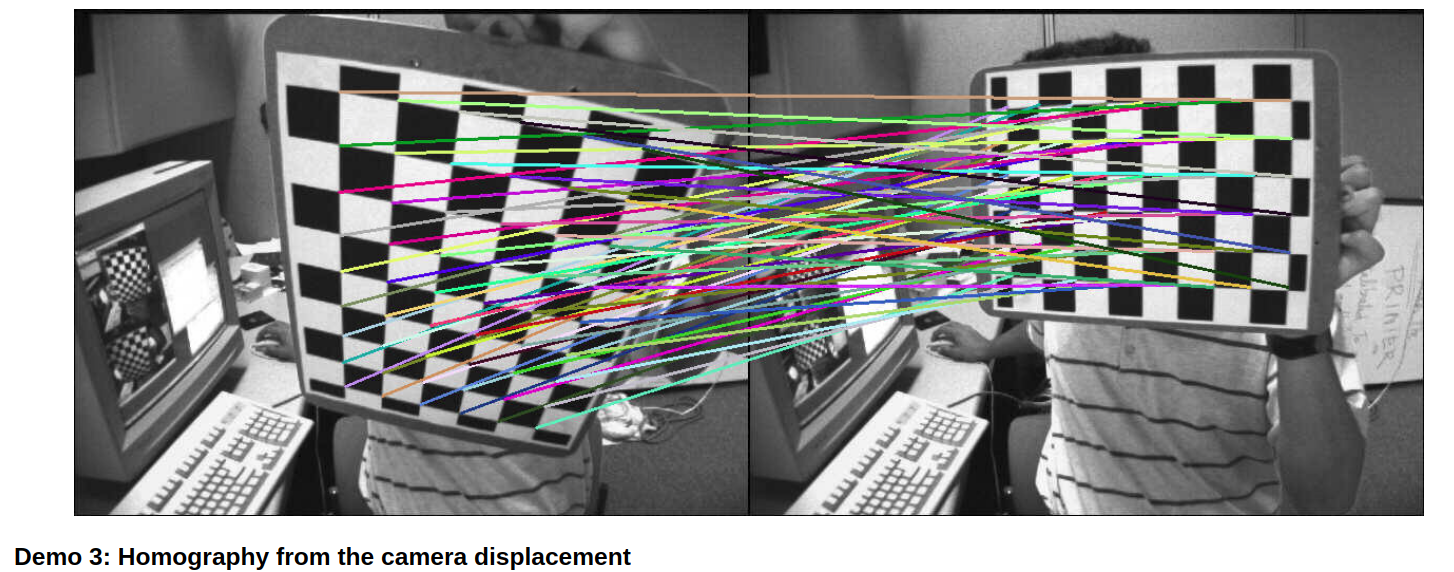
\includegraphics[width=\linewidth,natwidth=640,natheight=640]
  {fig/ref_imgs/feature_matchings.png}
  \caption{Feature Mathces}
	\label{fig:feature_matchings}
\end{figure}


\subsection{Brute-Force or FLANN} \label{sb_sc_}

\subsection{RANSAC} \label{sb_sc_ransac}

In reality, not all feature matches are correct and it is critical that we 
detect wrong ones as Least-Squares optimization that estimates the camera 
motion is sensitive to even small number of wrong matches. More technically,
we call these 
wrong matches \textit{outliers} (or \textit{false positives}). Hence, 
we need an algorithm to reject those outliers from \textit{inliers}. 
The most common way is to use RANSAC, which is an abbreviation to 
Random Sample Consensus. RANSAC is an interative algorithm which 
fits desired model with presence of outliers by selecting subset of dataset 
randomly and improving parameters of model each iteration. Note that 
RANSAC works 
well if at least half of the dataset contains inliers. 

\begin{figure}[H]
	\centering
	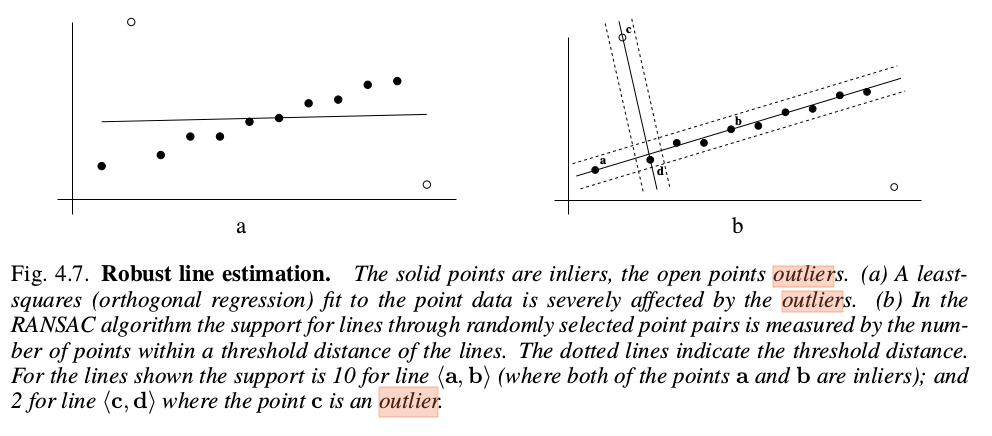
\includegraphics[width=\linewidth,natwidth=640,natheight=640]
  {fig/ref_imgs/line_ransac_outlier.png}
  \caption{Outlier Mathces}
	\label{fig:outlier_matches}
\end{figure}

In \ref{sb_sc_calibration}, we discussed how to model rotation and translation 
motion along with the intrinsic matrix. Parameteres that we aim to 
identify are elements of projection matrix in \ref{eq:proj_func_w_square_pix_skew}. 
Similarly, the model being fitted in RANSAC case is elements of a 
\textit{homography matrix}, 
which transforms a 2D image point to another 2D image point.
Remember that we have feature matches from image pairs. One of the pair is 
the transformed version of the other pair. 
We can model this relationship in the following way:

\begin{equation}
  k
  \begin{bmatrix}
    u_i' \\ v_i' \\1
  \end{bmatrix}
  =
  \mathbf{H}
  \begin{bmatrix}
    u_i \\ v_i \\1
  \end{bmatrix}
  =
  \begin{bmatrix}
    h_{00} & h_{01} & h_{02} \\
    h_{10} & h_{11} & h_{12} \\
    h_{20} & h_{21} & h_{22}
    \end{bmatrix}
  \begin{bmatrix}
      u_i \\ v_i \\1
    \end{bmatrix}
  \end{equation}\label{eq:homography_full}

The goal is to fit parameters of $\mathbf{H}$ with the selected subset of 
the matching and our assumption is majority of selected point matchings 
should be inliers. In this way, we can easily detect ourliers by testing 
whether they fit to model parameters or not. To make \ref{eq:homography_full} 
more obvious, we form linear system of equations:

\begin{equation}
\underbrace{
\begin{bmatrix}
  u_i & v_i & 1 & 0 & 0 & 0 & -u_i'u_i & -u_i'v_i -u_i'\\
  0 & 0 & 0 & u_i & v_i & 1 & -v_i'u_i & -v_i'v_i -v_i'
\end{bmatrix}}_{\mathbf{A}}
\underbrace{
\begin{bmatrix}
    h_{00} \\ h_{01} \\ h_{02} \\ h_{10} \\ h_{11} \\ h_{12} \\ h_{20} \\ h_{21} \\ h_{22}
\end{bmatrix}}_{\mathbf{h}}
= 
\begin{bmatrix}
  0\\0
\end{bmatrix}
\end{equation}

First step of RANSAC is to select a subset that contains 
minimum number of matching points to 
determine parameters of the model. In homography $\mathbf{H}$ case, we need at least 
4 point pairs $(\mathbf{p}=(u_i,v_i),\mathbf{q}=(u_i',v_i'))$ to solve 
this linear system of equation. However, due to the noise, we require more than 
4 point pairs but this makes the problem over-determined. Therefore, 
we can only find an approximate solution by solving least squares problem:
It is also good idea to optimize with all matching points and use 
the estimated parameters as a initial guess for the optimization 
which we perform for the subset. With all that being said, we minimize the 
\textit{algebraic distance error}:

\begin{equation}
\argmin_h || \mathbf{Ah-0}||^2.
\end{equation}

In the second step, 
after estimating $\mathbf{h}$ paramaters, we test every matchings that are 
outside the subset which randomly selected at the first step whether 
they fit to the model with the certain $\mathbf{d}$ threshold we define:

\begin{equation}
  ||\mathbf{q} - \mathbf{H}\mathbf{p}||_2 > \mathbf{d} 
\end{equation}

In the third step, we include the points 
that passed our test procedure in the second step into our subset. In the 
forth step, we have another test. In this test, we check whether the number of 
matching points in our subset is large enough to prove that we include 
majority of the inliers. If not, we go back to first step and repeat the 
whole process again until we fulfill the fourth step. Here is the pseudo code 
that summarize the algorithm:

\begin{algorithm}[H]
  \caption{Rejecting outlier matches with RANSAC}\label{algo_ransac}

  \textbf{Input} \\
    \hspace*{\algorithmicindent}\textbf{S}: the smallest number of points\\
    \hspace*{\algorithmicindent}\textbf{N}: the number of iteration\\
    \hspace*{\algorithmicindent}\textbf{d}: the threshold used to identify a point which fits the model\\
    \hspace*{\algorithmicindent}\textbf{T}: the number of nearby points to notify that there is a good fit\\
  \textbf{Output} \\
    \hspace*{\algorithmicindent}\textbf{C}: the (consensus) set of inliers \\
  \begin{algorithmic}[1]

    \Procedure{RANSAC}{\textbf{S,N,d,T}}\\
      \While{iterations $<$ \textbf{N}}
      \State select random sample subset of \textbf{S} points
      \State estimate parameters to fit homography with \textbf{S}
      \ForEach {points outside \textbf{S}}
        \State calculate error between estimated point and measured point
        \If {error $<$ \textbf{d}}
          \State add point into \textbf{S}
        \EndIf
        \If {\textbf{S} $>$ \textbf{T}}
          \State return \textbf{C} $=$ \textbf{S}
        \EndIf
      \EndFor
      \EndWhile
    \EndProcedure
  \end{algorithmic}

\end{algorithm} \label{algo:ransac}

As it is seen in \ref{algo:ransac}, there are number of empiric parameters 
that we need to define; $\mathbf{S,N,d,T}$. To make the algorithm as 
efficient as possible, these parameters must be chosen carefully. As we 
discussed, $\mathbf{S}$ is the subset of matchings that we randomly select and 
initial value should at least 4 so that we can solve the least 
squares problem. 

For $\mathbf{N}$, it is insufficient to iterate 
through every matching points. Thus, we at least select $\mathbf{N}$ 
number of mathcing points with respect to following condition:

\begin{equation}
  \mathbf{N} = log(1-p)/log(1-(1-\epsilon)^s)
\end{equation}

where $p=0.99$ is the probability of covering all inliers, $s$ is the 
minimum number of iteration that 
probability of choosing a subset with only outliers 
and $\epsilon$ is the probability that a matching is an outlier.

For $\mathbf{d}$, it is chosen empirically if distribution of outliers is unknown. If 
it is known, i.e, Gaussian with mean $\mu$ and $\sigma$, threshold should 
be $d=5.99\sigma^2$ so that there is a 95\% probability that the point is an inlier.

For $\mathbf{T}$, we might have a case that we reach expected ratio of inliers; thus 
we don't have to iterate through $N$ number of times. We can terminate it 
ealier if the following condition is satisfied:

\begin{equation}
  \mathbf{T} = (1-\epsilon)n
\end{equation}

where $n$ is the total number of matching points.

It is also important 
to note that estimated homography matrix corresponds the rotation and the 
translation that we want to calculate camera's trajectory. However, 
estimated homography matrix with the presence of outliers is not sufficient 
enough. Therefore, further optimization with is required to get more 
accurate rotation and translation with only inliers. We will discuss this 
optimization in the next section.


\section{Motion Estimation} \label{sc_motion_estim}

Motion estimation is the core part of the VO system. After 
feature extraction, feature matching and outlier rejection,
we finally are ready to compute $\mathbf{T}_{k, k+1}$ transformation matrix. 
This transformation matrix corresponds to relative camera motion between 
two images that is recorded in different poses (figure-\ref{fig:transformation_ij}).
Let's assume; we have 
consecutive camere poses $\mathbf{x}_k^c = [\mathbf{p}_k^c, \mathbf{q}_k^c]$ and 
$\mathbf{x}_{k+1}^c = [\mathbf{p}_{k+1}^c, \mathbf{q}_{k+1}^c]$ where 
$\mathbf{p}^c = [p_x, p_y, p_z]^T$ is the position of the camera in $\R^3$
and $\mathbf{q}^c = [q_w, q_x, q_y, q_z]^T$ is 
the orientation of the camera in quaternion form in $SO(3)$. 
Notice that, in camera model chapter 
\ref{cp_cam_models}, we used rotation matrix to represent orientations, 
which made it covenient to combine intrinsic matrix and extrinsic matrix 
(rotation and translation) into a single projection matrix 
(refer to notation \ref{eq:simplyfied_proj_func})
so that 
we optimize for paramaters of the single matrix. On the other hand, when 
estimating relative motion, we use quaternions to represent orientations, 
which is less intuitive way but 
has certain advantage over rotation matrix such as requiring less storage.
Additionally, we can represent the transformation 
$\mathbf{T}_{k,k+1}$ $(= [\mathbf{t}_{k,k+1},\mathbf{q}_{k,k+1}])$ between two camera poses 
$(\mathbf{x}_k,\mathbf{x}_{k+1})$ with the rotation $\mathbf{q}_{k,k+1}$ in $SO(3)$  
and the translation $\mathbf{t}_{k,k+1}$ in $\R^3$.

\begin{figure}[H]
	\centering
  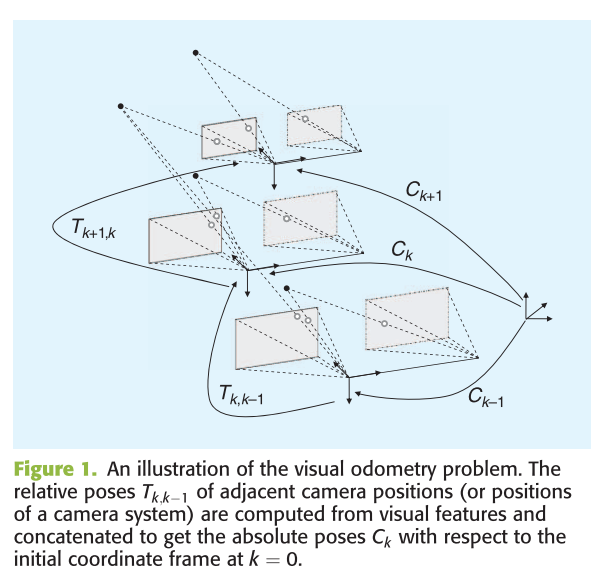
\includegraphics[width=0.7\linewidth,natwidth=640,natheight=640]
  {fig/ref_imgs/transformation_ij.png}
  \caption{GIVE EX FOR TRANSFORMATION TWO CAM POSES Transformation between Two Images}
	\label{fig:transformation_ij}
\end{figure}

That being said, one can formulate the transformation $\mathbf{T}$ 
between two camera pose. Let's first find the camera position:

\begin{equation}
  \mathbf{p}_{k+1} = 
  \mathbf{q}_{k,k+1} \otimes \mathbf{p}_k^c \otimes \mathbf{q_{k,k+1}}^* + 
  \mathbf{t}_{k,k+1}
\end{equation}

where $\mathbf{q}_{k,k+1} \otimes \mathbf{p}_k \otimes \mathbf{q_{k,k+1}}^*$ is the 
\textit{hamilton product} that is used to rotate the camera position at the $k^{th}$ pose 
and $\mathbf{t}_{k,k+1}$ is 
the simple vector addition that is used to translate the camera position. Next, 
the camera orientation can be found as follows:

\begin{equation}
  \mathbf{q}_{k+1} = 
  \mathbf{q}_{k,k+1} \otimes \mathbf{q}_{k}^c double-check product order
\end{equation}

where $\mathbf{q}_{k,k+1} \otimes \mathbf{q}_{k}$ is the product of two 
quaternions that the former is the rotation and that the latter is the orientation 
of the camera at the $k^{th}$ pose.

\begin{figure}[H]
	\centering
  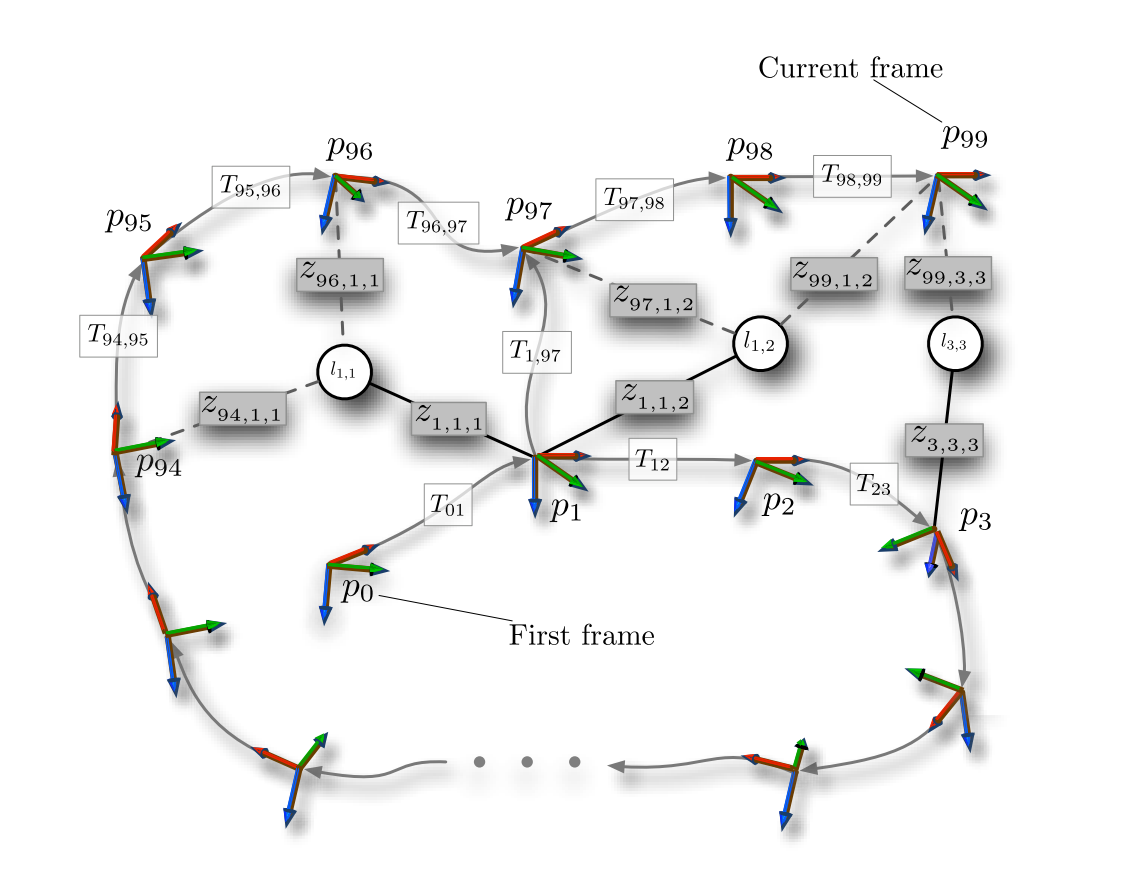
\includegraphics[width=0.7\linewidth,natwidth=640,natheight=640]
  {fig/ref_imgs/cam_trajectory.png}
  \caption{Camera Trajectory}
	\label{fig:cam_trajectory}
\end{figure}


The ultimate goal in VO is to compute transformation
$\mathbf{T}_{k,k+1}=[\mathbf{t}_{k,k+1},\mathbf{q}_{k,k+1}]$ in multiple consecutive 
images and concatenate them to build a trajectory of the camera.
As a consequence, we can track any agent on which the camera is placed rigidly. 
For example, concatenated transformation $\mathbf{T}_{0:n}$ 
can be used to calculate $n^{th}$ camera pose that is relative to the initial pose:


\begin{equation}
  \mathbf{p}_{n}^c = 
  \mathbf{q}_{n, n-1} \otimes (\dots
  (\mathbf{q}_{2,1} \otimes
  (\mathbf{q}_{1,0} \otimes \mathbf{p}_0^c \otimes \mathbf{q_{1,0}}^* + \mathbf{t}_{1,0})
  \otimes \mathbf{q}_{2,1}^* + \mathbf{t}_{2,1})
  \dots) \otimes \mathbf{q}_{n, n-1}^* +\mathbf{t}_{n, n-1} 
\end{equation}

\begin{equation}
  \mathbf{q}_{n}^c = 
  \mathbf{q}_{n,n-1} \otimes \dots \otimes \mathbf{q}_{2,1} \otimes \mathbf{q}_{1,0} \otimes \mathbf{q}_{0}^c 
\end{equation}

To find transformation, we take advantage of the feature points as they can 
inform us how the camera moves if we detect them in multiple image frames.
All the feature extraction and feature matchings are performed so that we 
can compute relative motion.
Similar to projection matrix \ref{eq:proj_lsq} in camere calibration, we utilize 
the least squares method for estimating the best approximate transformation information
due to the noise. Several methods available in literature create 
relationship between feature points that we detect across different image frames and 
we will discuss it in the next section.

\subsection{Relative Camera Pose Estimation Techniques}
\label{sb_sc_relative_camera_pose_estimation_techniques}

The reason we have different kinds of way to compute transformation arises from 
the cost function we define in least squres problem. In the end, all we wish to 
find a good model for our optimization problem so that we minimize the error.
The design choice for cost function comes from the fact that we either use 
2D keypoints, 3D point clouds (if we back-project 2D keypoints using 
calibrated projection matrix), or both.
Therefore, in VO literature, 
there are 3 different cost functions for modeling the least problem:
\begin{itemize}
  \item 2D-to-2D correspondences,
  \item 3D-to-2D correspondences,
  \item 3D-to-3D correspondences.
\end{itemize}
The 2D term refers to 2D points that are in the image plane and that we call 
them keypoints in section-\ref{sb_sc_feature_descriptor}. 
Whereas the 3D term refers to 3D points that are in the Camera Coordinate 
System and that we call them point clouds in section-\ref{sb_sc_feature_descriptor}.

NOTE: define keypoints and point clouds term if it is not defined in the feature extraction section.

Note that this thesis does not engage with 2D-to-2D correspondences method since it is 
used in monocular camera; thus it will not be discussed here. On the other hand, 
we will discuss and compare 3D-to-2D correspondences and 3D-to-3D correspondences. 
In the motivation chapter \ref{cp_motivation}, 
I state the reasons why I chose 3D-to-3D even though it is not a common choice 
in VO literature.


\subsubsection{3D-to-2D Correspondences}

Rememeber that,
after feature matching step for the consecutive image frames, we have only
2D-to-2D keypoint correspondences information and 
the transformation which we wish to compute is in $\R^3$. Therefore, we require 
transformation involving in 3D feature points.
That being said, we can estimate transformation 3D-to-2D Correspondences in four steps:

\begin{enumerate}
  \item back-project $k+1^{th}$ 2D keypoint to a 3D feature point
  \item back-transform the back-projected 3D feature point
  \item reproject the back-transformed 3D feature point onto $k^{th}$ keypoint
  \item minimize 2D \textit{reprojection error} along with all feature matches
\end{enumerate}

\begin{figure}[H]
	\centering
  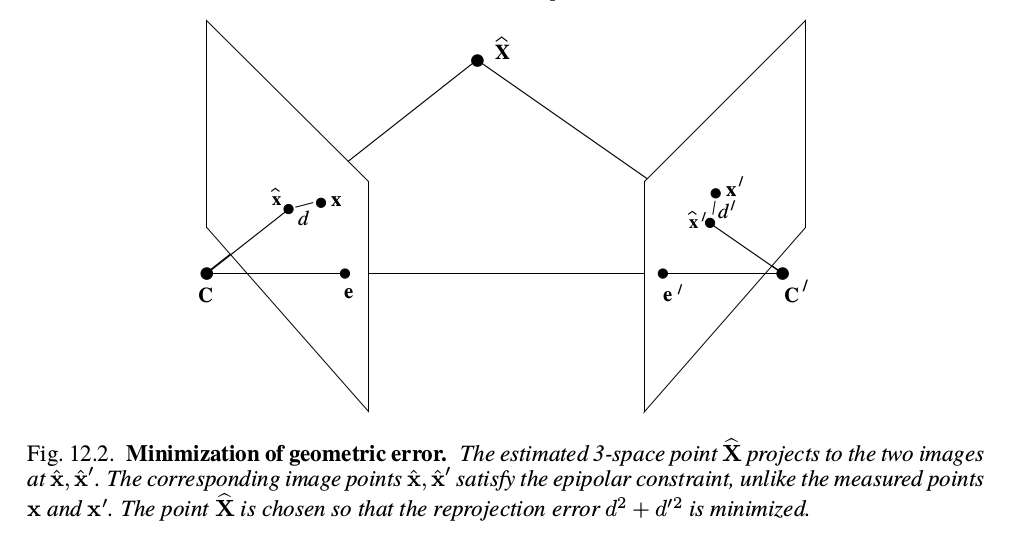
\includegraphics[width=0.7\linewidth,natwidth=640,natheight=640]
  {fig/ref_imgs/min_euclidean_error.png}
  \caption{Minimize Reprojection Error}
	\label{fig:min_geometric_error}
\end{figure}


To illustrate the 
situation more clearly, let's assume we have a 3D feature point 
$\mathbf{X}_i=[x, y, z]^T$ in Camera Coordinate System and we measure 
the projections of this exact feature point as 2D keypoint features, 
$\mathbf{x}_i^k=[u_i^k,v_i^k]^T$ and $\mathbf{x}_i^{k+1}=[u_i^{k+1}, v_i^{k+1}]^T$ 
on subsequent camera poses $k^{th}$ and $k+1^{th}$ respectively. What we also know is that 
we can back-project measured 2D keypoints to 3D feature points using projection 
matrix \ref{eq:simplyfied_proj_func_1} that we estimated in calibration process. 
Note that, since we measure 3D feature points with respect to Camera coordinate system, 
we are not interested in extrinsic matrix but only intrinsic. Now, 
let's write again projection function that converts 3D feature 
points to 2D image keypoints:
$
\mathbf{x}_i = 
  \mathbf{K}\mathbf{X}_i
  $.
One can also back-project 2D image keypoints to 3D feature points:
$
  \mathbf{K}^T\mathbf{x}_{i} = 
  \mathbf{X}_{i} 
  $.

Now, we can formulate the four steps of 3D-to-2D correspondences as follows:

\begin{enumerate}
  \item $\mathbf{X}_{i}^{k+1} = \mathbf{K}^T\mathbf{x}_{i}^{k+1}$
  \item $\mathbf{X}_i^{k'} = 
    \mathbf{q}_{k,k+1}^* \otimes (\mathbf{X}_i^{k+1} - \mathbf{t}_{k,k+1}) \otimes \mathbf{q}_{k,k+1}$
  \item $\mathbf{x}_i^{k'} = \mathbf{K}\mathbf{X}_i^{k'}$
  \item minimize $\sum_i||\mathbf{x}_i^k - \mathbf{x}_i^{k'}||_2^2$
\end{enumerate}

The second and third steps can be encapsulated to a function $f$ so that 
we formulate the whole optimization problem in the following form:

\begin{equation}
  \argmin_{\mathbf{T} = [\mathbf{t}_{k,k+1}, \mathbf{q}_{k,k+1}]} = 
  \sum_i||\mathbf{x}_i^k - f(\mathbf{T}, \mathbf{X}_i^{k+1})||^2_2
\end{equation}

This method works considerably well in practice. In VO literature \cite{}, 
it is also reported that it performs better than 3D-to-3D correspondences.

\subsubsection{3D-to-3D Correspondences}

Another way of modeling the cost function is to utilize only 3D feature point 
correspondences and one can estimate transformation with 3D-to-3D correspondences in three steps:

\begin{enumerate}
  \item back-project both $k^{th}$ and $k+1^{th}$ 2D keypoints to 3D feature points
  \item back-transform back-projected $k+1^{th}$ 3D feature point
  \item minimize 3D \textit{euclidean distance} along with all feature matches
\end{enumerate}

\begin{figure}[H]
	\centering
  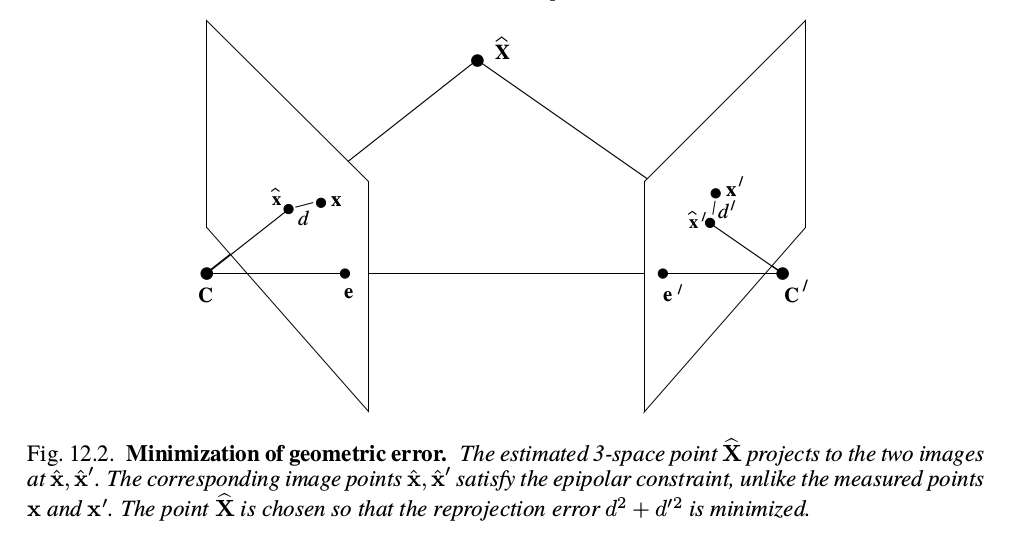
\includegraphics[width=0.7\linewidth,natwidth=640,natheight=640]
  {fig/ref_imgs/min_euclidean_error.png}
  \caption{Minimize Euclidean Error}
	\label{fig:min_euclidean_error}
\end{figure}


Similar illustrations that we previously did for 3D-to-2D correspondences applies 
for the 3D-to-3D correspondences as well but only with few changes. 
Let's again assume that we have two corresponding 2D keypoint features,
$\mathbf{x}_i^k$ and $\mathbf{x}_i^{k+1}$. However, rather minimizing error on 
2D image plane, we want to minimize them on 3D Camera coordinate system. Therefore, 
we need to back-project both keypoint features. With that in mind, 
we can formulate the three steps of 3D-to-3D correspondences as follows:

\begin{enumerate}
  \item $\mathbf{X}_{i}^{k+1} = \mathbf{K}^T\mathbf{x}_{i}^{k+1}$ and 
    $\mathbf{X}_{i}^{k} = \mathbf{K}^T\mathbf{x}_{i}^{k}$ 
  \item $\mathbf{X}_i^{k'} = 
    \mathbf{q}_{k,k+1}^* \otimes (\mathbf{X}_i^{k+1} - \mathbf{t}_{k,k+1}) \otimes \mathbf{q}_{k,k+1}$
  \item minimize $\sum_i||\mathbf{X}_i^k - \mathbf{X}_i^{k'}||_3^2$
\end{enumerate}

The second step can be encapsulated to a function $g$ to form the optimization 
problem:

\begin{equation}
  \argmin_{\mathbf{T} = [\mathbf{t}_{k,k+1}, \mathbf{q}_{k,k+1}]} = 
  \sum_i||\mathbf{X}_i^k - g(\mathbf{T}, \mathbf{X}_i^{k+1})||^2_3
\end{equation}

In VO literature, this method is usually discarded since 
it performs poorly comparing to 3D-to-2D correspondences.

NOTE: State why it works poorly? Is it bc back-projected 3D feature point more noisy?

% ***************************CP3-MOTIVATION***************************
\chapter{Motivation} \label{cp_motivation}

% ***************************CP4-CoVO***************************
\chapter{An Error-Aware RGB-D Visual Odometry} \label{cp_covo}

REMEMBER TO DRAW X,Y COORD. WRT CAM. COORD WITH RIGHT HAND FOR KINECT!

\section{Modeling Spatial Uncertainty} \label{sc_spatial_uncertainty}

\begin{figure}[H]
	\centering
  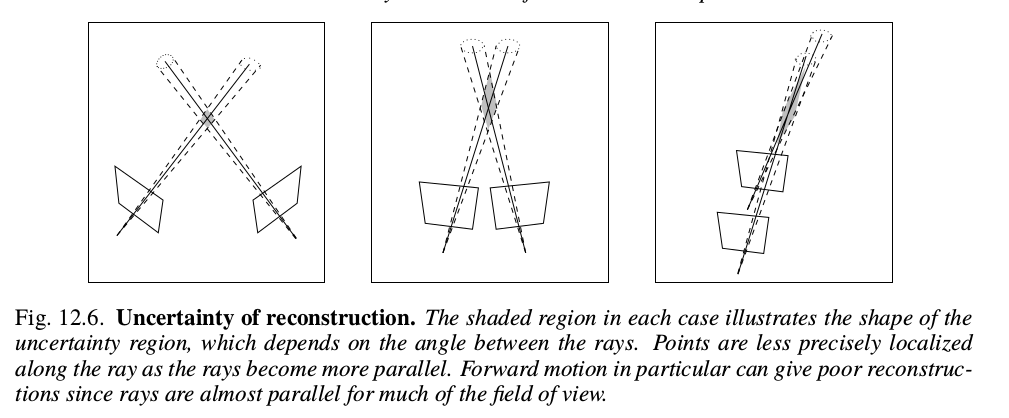
\includegraphics[width=0.7\linewidth,natwidth=640,natheight=640]
  {fig/ref_imgs/uncertainty_matching.png}
  \caption{Uncertainty of Feature Matchings}
	\label{fig:uncertainty_matching}
\end{figure}




\subsection{Kinect Calibration} \label{sb_sc_kinect_calibration}

\section{Weighted Least-Squares Optimization} \label{sc_weighted_lsq}

\section{Covariance Estimation} \label{sc_covariance_estim}

% ***************************CP5-EVALUATION***************************
\chapter{Evaluation} \label{cp_evaluation}

% ***************************CP6-CONCLUSION***************************
\chapter{Conclusion} \label{cp_conc}

% ***************************CP7-EVALUATION***************************
\chapter{Reference} \label{cp_ref}


% ***************************CP7-EVALUATION***************************
\chapter{Appendices} \label{cp_appendices}

\section{Rigid-Body Transformations} \label{sc_rigid_body_transformations}


\section{Least Squares}\label{sc_least_squares}

Throughout this thesis, least squares method empowered many different components 
of out VO system, 
such as camera calibration, RANSAC and most importantly motion estimation, 
Therefore, we will discuss underlying principles of least squares method in this section.

Ultimately, error minimization is an 
operation which wish to get the maximum likelihood of the function. To do so,
we search the most
likely state configuration as close as possible to its exact and ideal solution. 
In the case of any optimization problems,
the goal is to find interesting points, such as local/global
maximum or local/global minimum, on the \textit{objective}
\textit{function}. However, due to the
non-linearity and noise in measurements, one can only approximate a solution.
One way to solve such problems is to generate a quadratic model of 
the objective function and iterate
through the function using \textit{Newton's methods}. 
For example,
an optimal solution (or an interest point)
Figure-\ref{fig:lsq_multivariable_function_example} is at the local
minimum of the function that is highlighted as a red point cloud.

\begin{figure}[H]
	\centering
	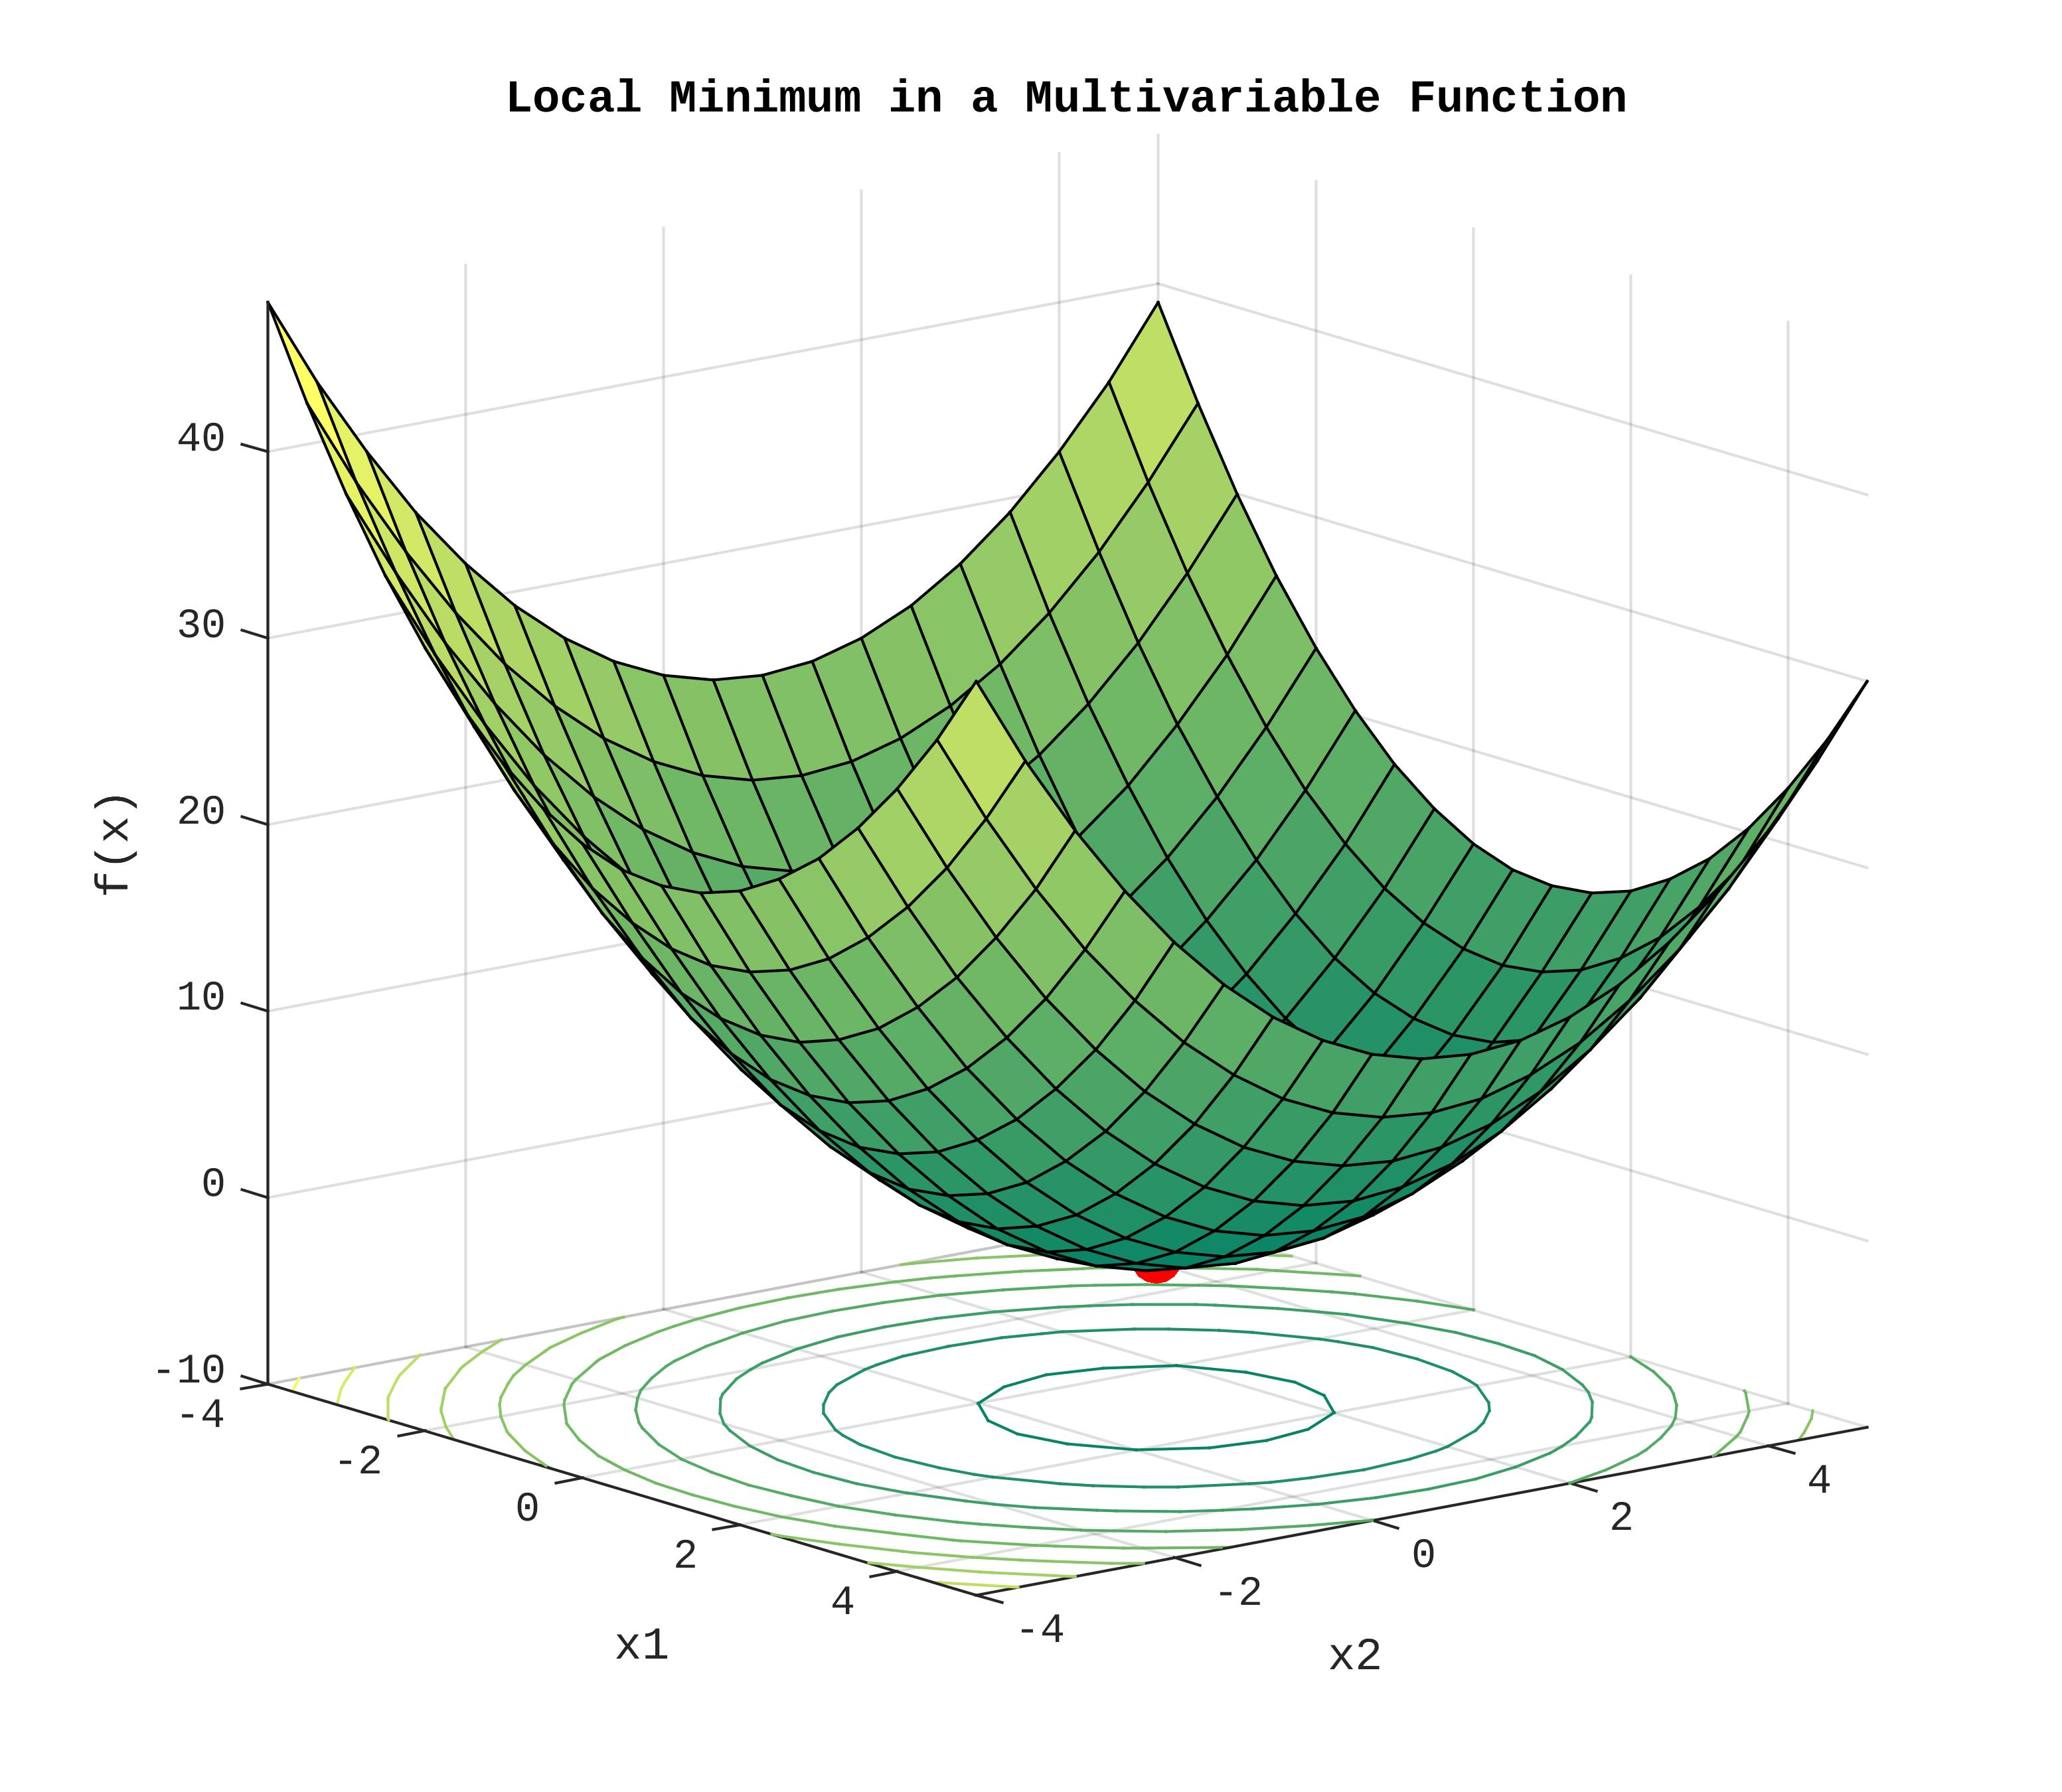
\includegraphics[width=\linewidth,natwidth=640,natheight=640]
	{fig/lsq_multivariable_function_example.jpg}
	\caption{Local Minimum at a Quadratic Function}
	\label{fig:lsq_multivariable_function_example}
\end{figure}


In optimization literature,
there are many versions of Newton's method 
and they all try to find the
local maximum/minimum in the most efficient and accurate way.
However, in the end, they all solve the problem
with the \textit{gradient descent} manner.
%the approximated Hessian function, is one of them and we will be using
%it in our slam algorithm.
To elaborate the problem, we provide a regression example 
which can be infact solved with linear least squares techniques but it can serve 
as a simple toy example throughout our explainations.

Suppose that we have a model function $g(x;a)$. However,
we don't know what the $x=(x_1,x_2)$ coefficients (so-called
\textit{optimization} \textit{parameters}) are and we can only
plug $a$, which is the \textit{independent} variable, into the
\textit{model} $S$ to see
how the output of the model changes given the independent variable. 

\begin{figure}[H]
	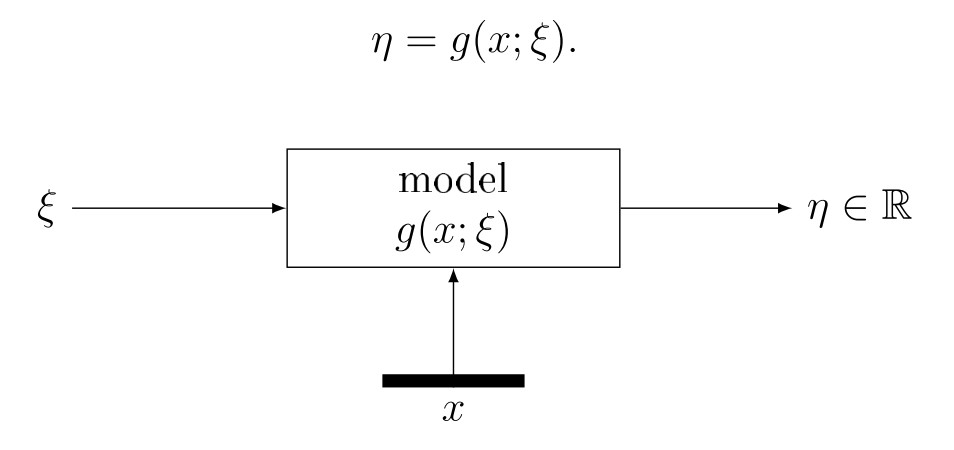
\includegraphics[width=0.8\linewidth,natwidth=640,natheight=640]
	{fig/lsq_model.jpg}
	\centering
	\caption{Least Square Model}
	\label{fig:lsq_model}
\end{figure}



\begin{gather}
\xi = a \text{ (independent variable)} \in \R \\
\eta = S \text{ (dependent variable)} \in \R
\label{eq:lsq_model_variables}
\end{gather}

\begin{equation}
S = g(x;a) := x_1 + x_2a \quad 
\text{where} \quad 
x=(x_1,x_2) \in \R^2
\label{eq}
\end{equation}


To see this effect, 
we draw a graph that is shown in
Figure-\ref{fig:lsq_curve_fit_measurements}.

\begin{figure}[H]
	\centering
	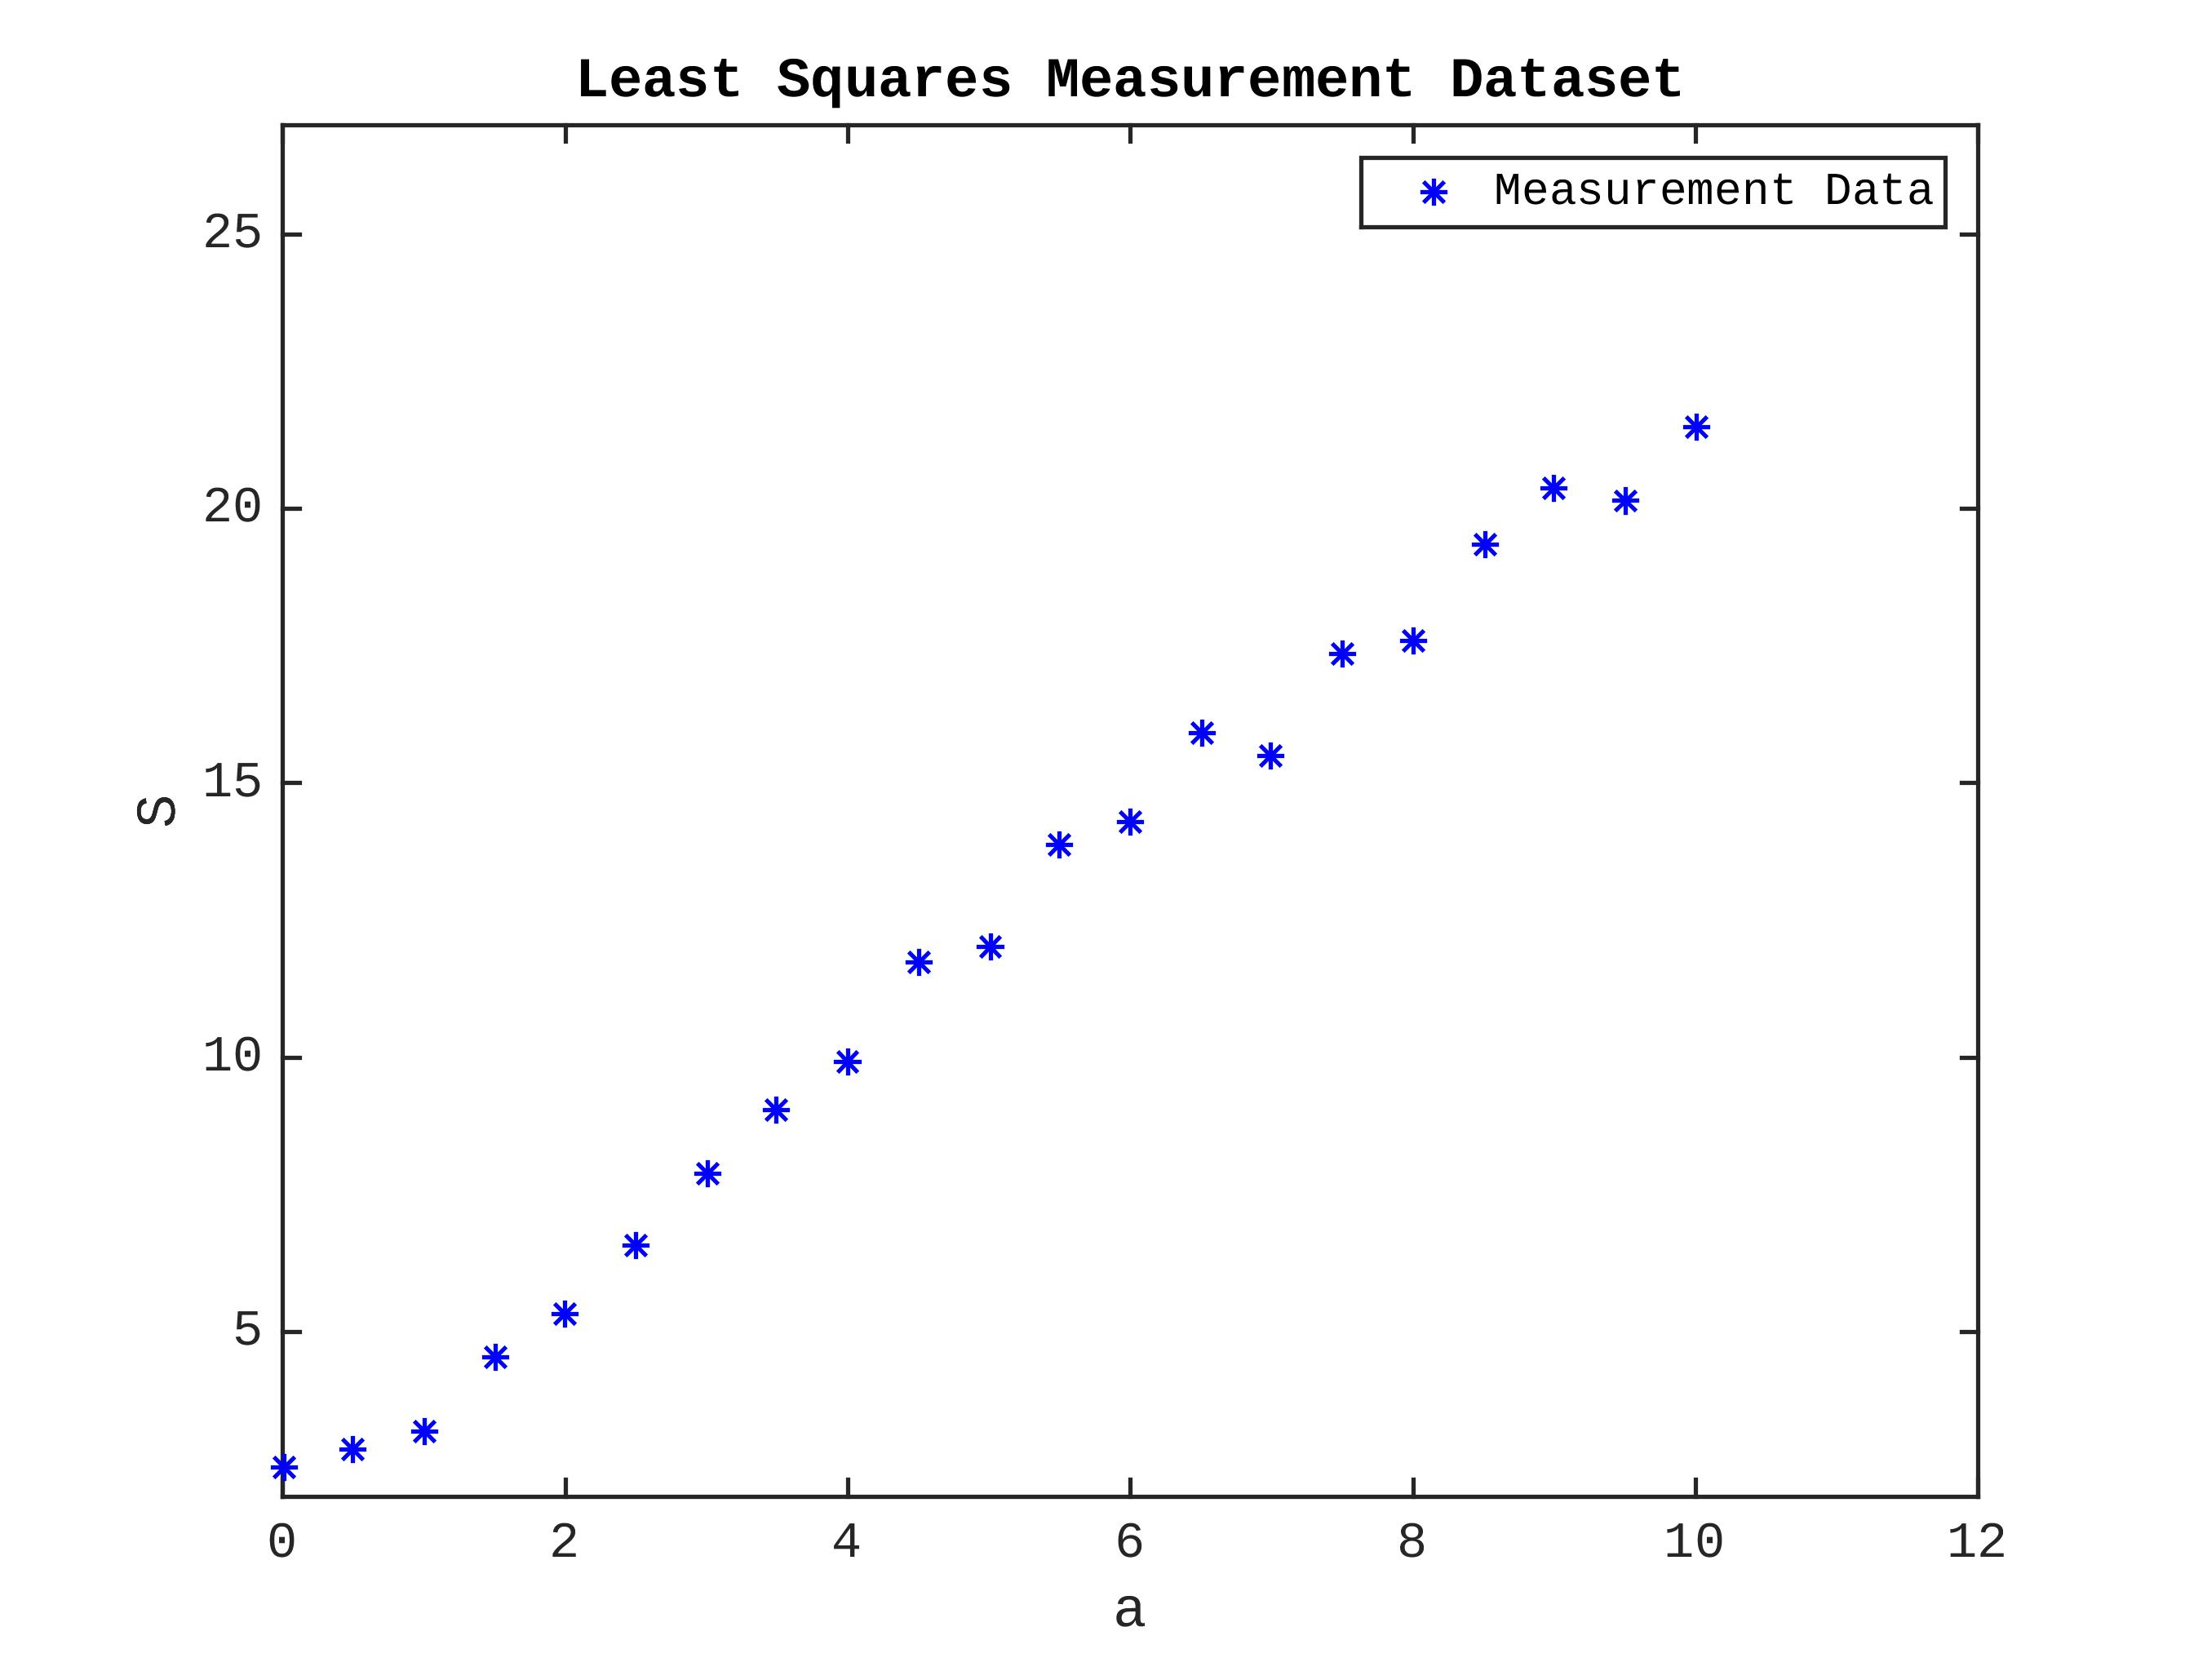
\includegraphics[width=\linewidth,natwidth=640,natheight=640]
	{fig/lsq_curve_fit_measurements_v2.jpg}
	\caption{Least Squares Measurements}
	\label{fig:lsq_curve_fit_measurements}
\end{figure}


Our goal is now to find a function, which will fit this
dataset. This is a typical least squares curve fitting problem.
In this problem, we construct a \textit{residuals function} $r_i(x)$ by providing
error values between model estimation $g(x;a_i)$ and dependent
variable $S_i$. In this case, the dependent variable 
represent the real world
measurements and the residuals function represents the error between the estimated value and measurement value. 

\begin{equation}
r_i(x) := g(x;a_i) - S_i \qquad \text{ for }  i = 1,\dots,m.
\label{eq:}
\end{equation}

The residuals function is usually squared to magnify larger error effect:

\begin{equation}
\begin{aligned}
F(x) & := \sum_{i=1}^{m} \vert r_i(x) \vert^2 = 
\sum_{i=1}^{m} \vert g(x;a_i) - S_i \vert^2 =
\sum_{i=1}^{m} (g(x;a_i) - S_i)^2 \\
\label{eq}
\end{aligned}
\end{equation}

Now, one can use the sum of squared error function to calculate the most likely
configuration that can minimize the errors. 

\begin{equation}
X^* = \argmin_x F(x) = 
\sum_{i=1}^{m} (g(x;a_i) - S_i)^2, 
\quad x \in \R^2
\label{eq}
\end{equation}

At this point, the objective function is ready to be handed over to 
to any gradient decent based least squares solver. The method will try to find the
\textit{optimal} solution $X^*$ by minimizing the objective function.

\begin{equation}
\text{Minimize} \quad \sum_{i=1}^{m} (g(x;a_i) - S_i)^2, 
\quad x \in \R^2
\label{eq}
\end{equation}

To help our understanding, the objective function is drawn in
Figure-\ref{fig:lsq_sum_of_squared_error_function}.
As we can see, the based on the given $x=(x_1,x_2)$ values, 
the objective
function $F(x)$ behave as follows:

\begin{figure}[H]
	\centering
	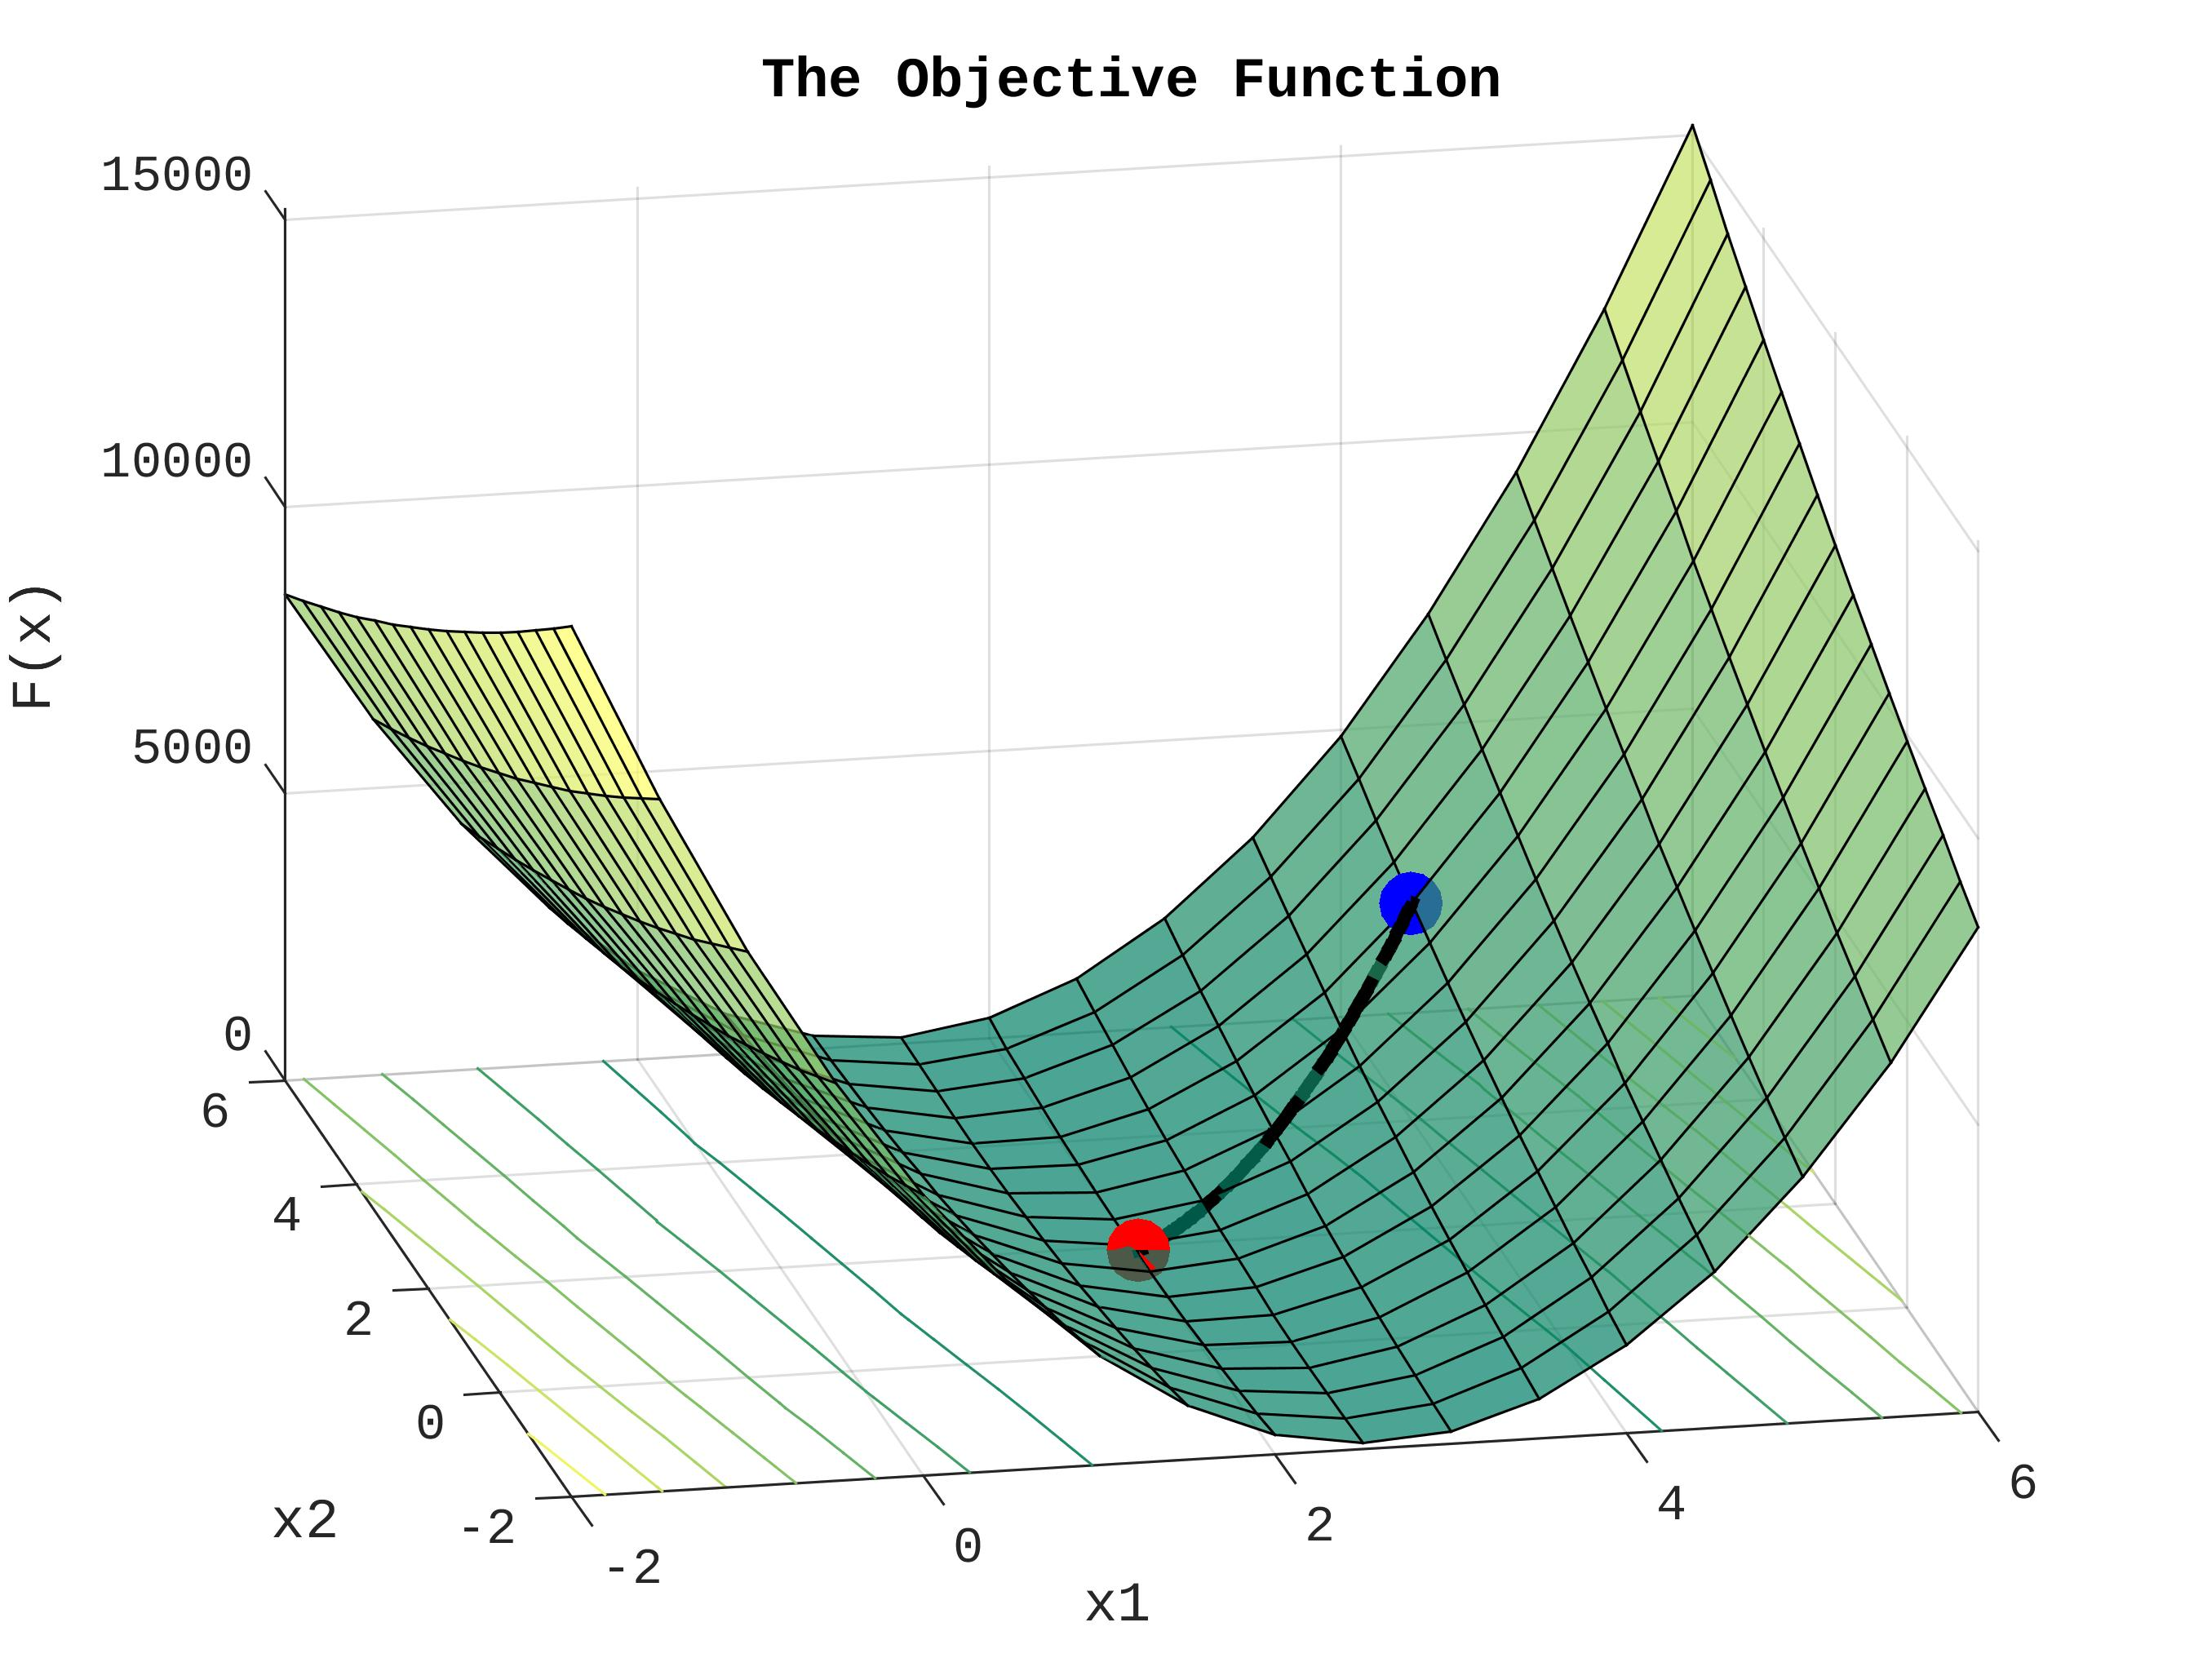
\includegraphics[width=\linewidth,natwidth=640,natheight=640]
	{fig/lsq_sum_of_squared_error_function_v2.jpg}
	\caption{Local Minimum at Sum of Squared Error Function}
	\label{fig:lsq_sum_of_squared_error_function}
\end{figure}

The initial guess for the optimization parameters at $x=(4,4)$, which
is highlighted as a blue color point cloud and 
the local minimum point, which is the interest point of ours, 
is highlighted with the red cloud. What the gradient descent method essentially 
does is to travel from the initial guess point to the nearest local minimum 
on the objective function. As we can see
that the descent is successfully performed and the optimization
operation results at $x=(1.9,2.1)$. 


If we now place the optimization variables into our model function, we
get the $g(x;a)=1.9+2.1a$ and a fitted line based on the given
dataset in
Figure-\ref{fig:lsq_curve_fit_operation}.

\begin{figure}[H]
	\centering
	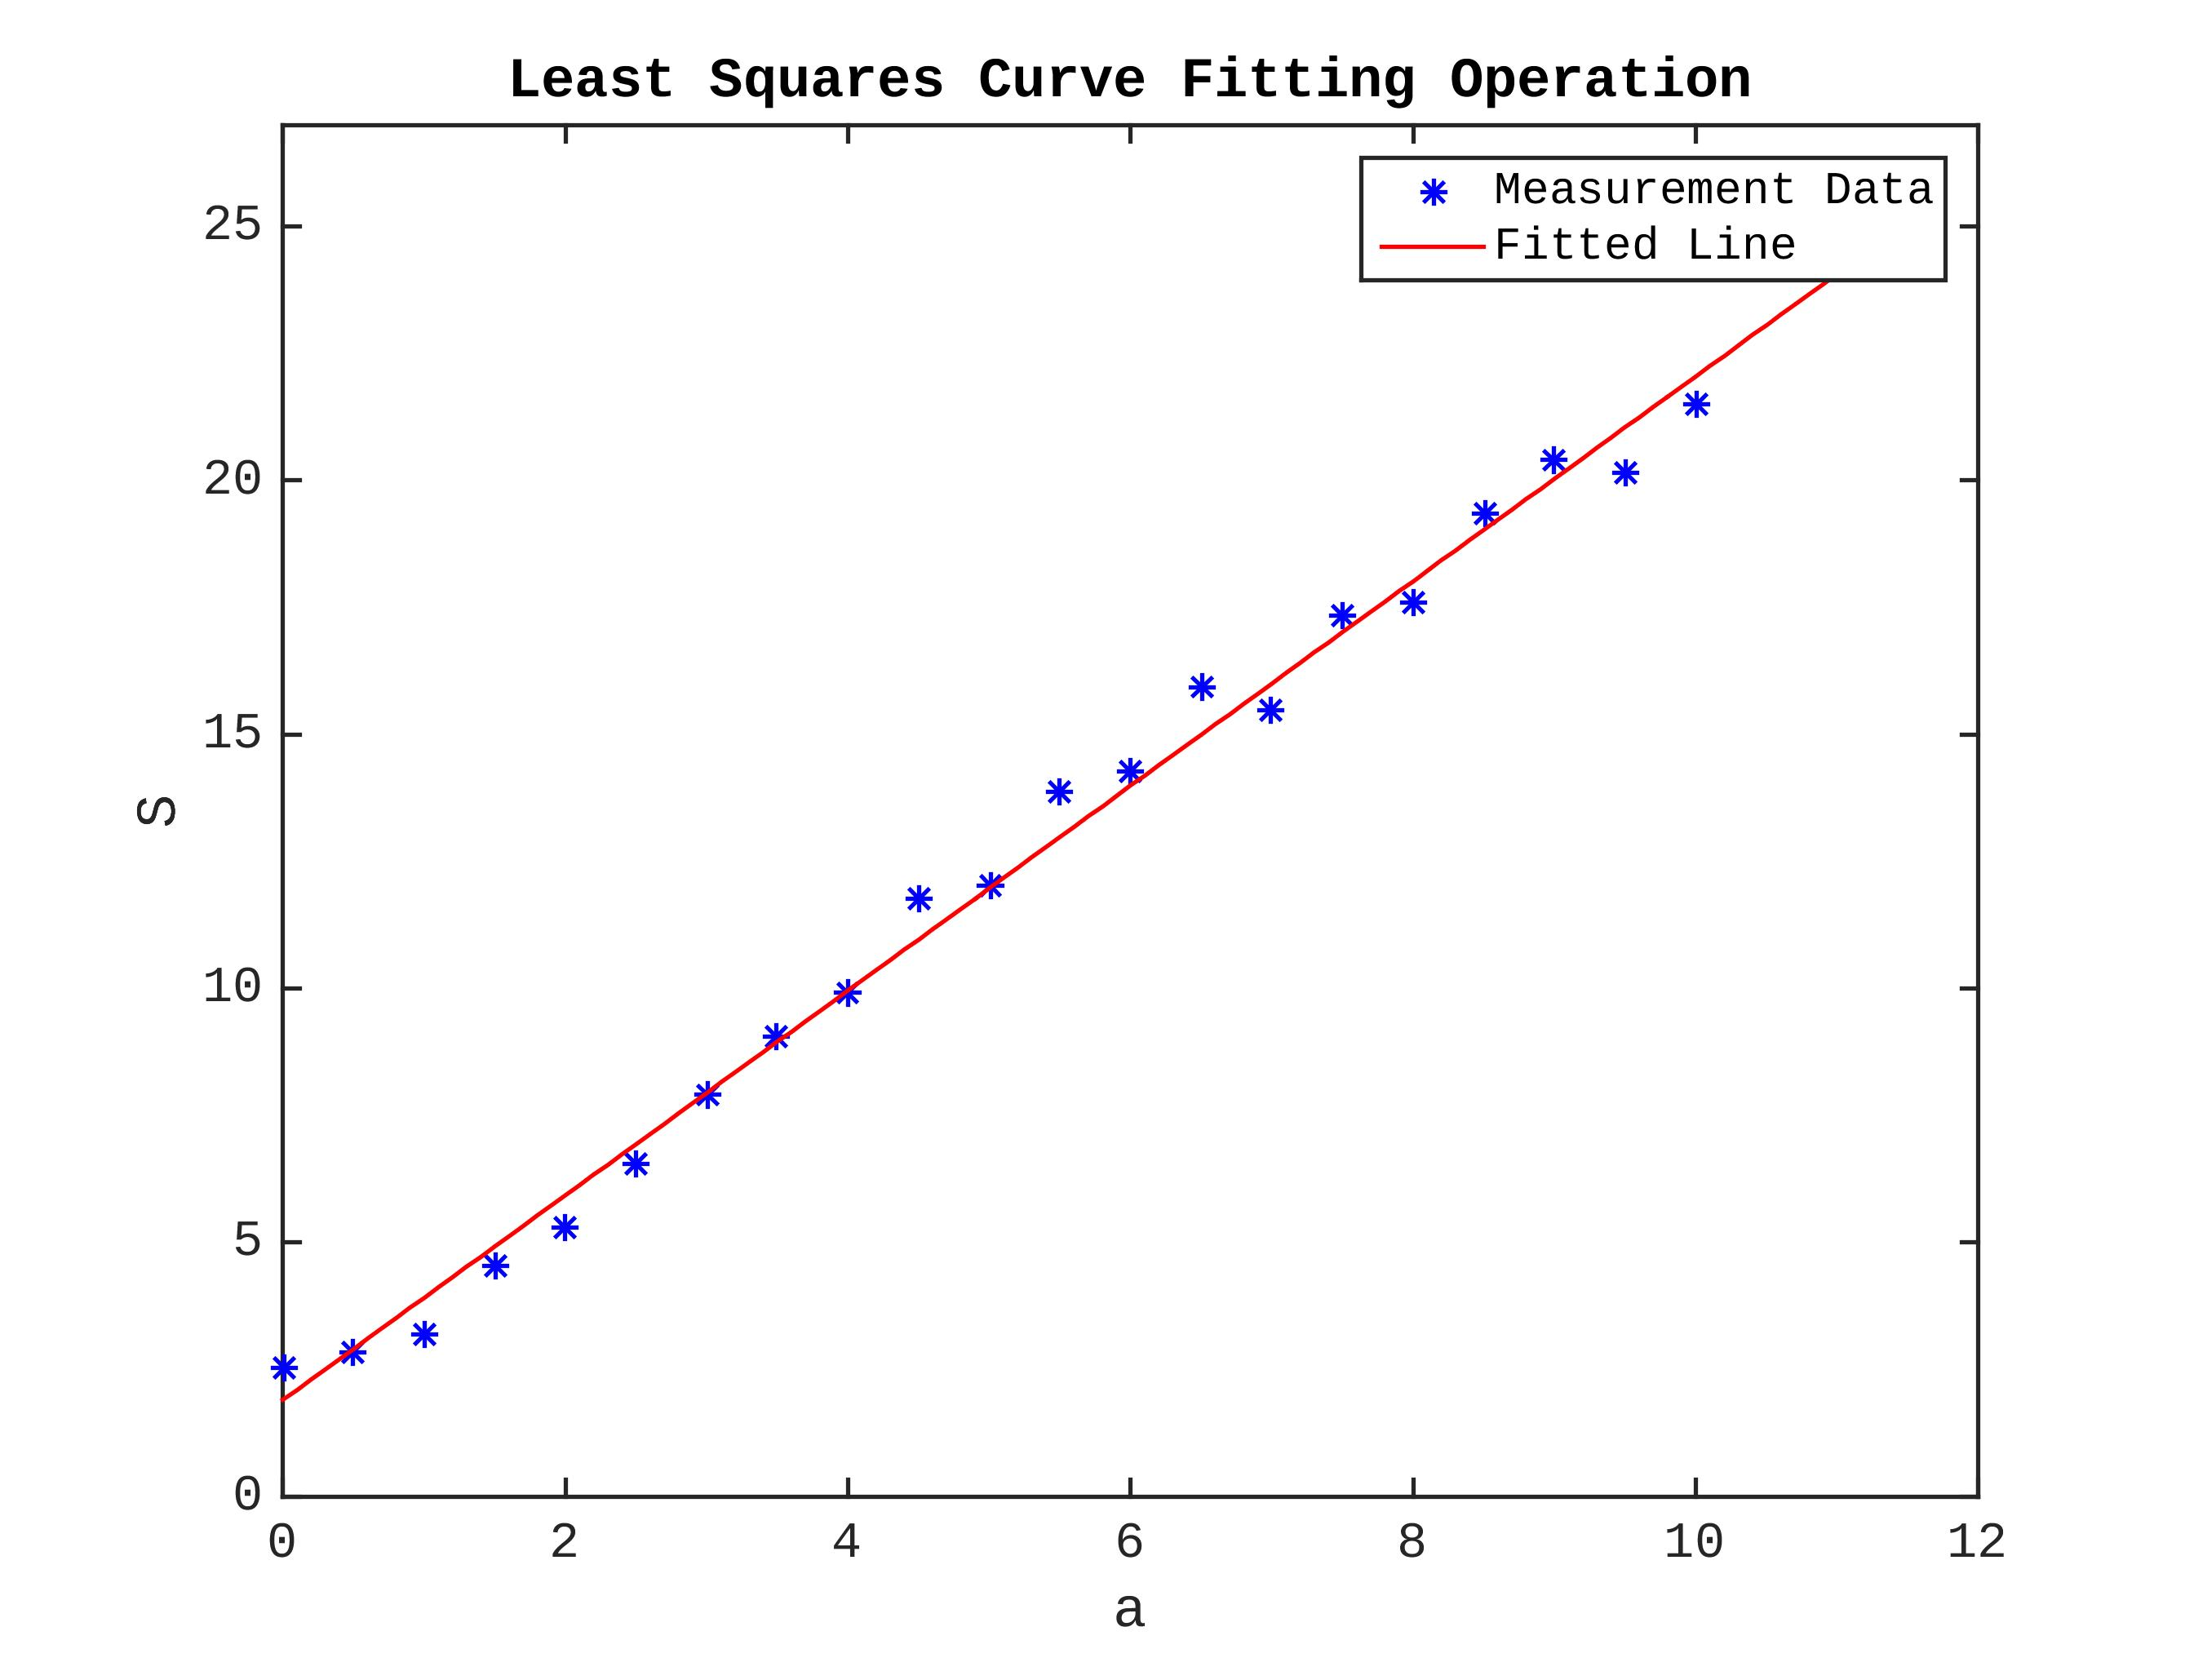
\includegraphics[width=\linewidth,natwidth=640,natheight=640]
	{fig/lsq_curve_fit_operation_v2.jpg}
	\caption{Least Squares Curve Fitting Operation}
	\label{fig:lsq_curve_fit_operation}
\end{figure}

Now that we have an intiution how least squares problems are solved 
by gradient descent methods, let's further discuss one of them.

\subsection{Gradient Descent}

In order to understand non-linear least square algorithms, 
we first need to look at how a gradient descent algorithm works. For instance; 
assuming that the objective function $F(x)$ is differentiable and its 
derivative has the following form:

\begin{equation}
  \nabla F(x) = F'(x) = \frac{\partial F(x)}{\partial x}
\end{equation}

Another fact about $F(x)$, considering above formula, is that its value will decrease 
in the direction of its negative derivative:

\begin{equation}
  \Delta x = - \frac{\partial F(x)}{\partial x}
\end{equation}

That being in mind, one can 
claim that if we iteratively travel through the function in the direction of its negative 
derivative, we would eventually reach to a nearest local minima with respect to the starting 
point. This is the fundamental idea behind gradient descent algorithm.
On the other hand, using its derivative directly does not ensure that 
we would reach to any local minima in some cases. Thus, a tuning factor so-called 
\textit{step length} $\alpha$ is used to adjust the size of length:

\begin{equation}
  \Delta x = -\alpha \frac{\partial F(x)}{\partial x}
\end{equation}



Assuming that we have an educated initial guess $x_0$ from which we start to search 
for a local minimum, we can describe the gradient descent algorithm as follows:

\begin{enumerate}
  \item take the derivative of $F(x)$ at the current $x_k$
  \item find the sufficient step length $\alpha$
  \item iterate $x_{k+1} = x_k - \alpha \frac{\partial F(x_k)}{\partial x}$ until it converges
\end{enumerate}

As we see, the gradient descent is a simple algorithm but it is an iterative 
approach that might require an exhaustive search operation if the initial 
guess is not given intellegently. Therefore, it can get very complicated 
if convergence speed and convergence success is considered. For this reason, 
there are many version of the algoritm that aims to solve in the most efficient 
manner.

\subsection{Levenberg-Marquardt}
Levenberg-Marquardt (LM) is one of most popular gradient descent based algoritm 
to solve least squares problem.


Assume that we have a $r(x)$ residuals function:

\begin{equation}
  r(x) := \begin{pmatrix} r_1(x) \\ \vdots \\ r_m(x) \end{pmatrix} \in \R^m
\end{equation}

To find a local maximum/minimum of the residuals function, we need to 
determine the first derivative and it 
$r'(x)$ appears in a special form, e.g., Jacobian:

\begin{equation}
  J(x) := \begin{bmatrix} \frac{\partial}{\partial x_j }r_i(x) \end{bmatrix}_{ij} 
  = 
  \begin{bmatrix} 
    \vertbar & & \vertbar \\
    \frac{\partial}{\partial x_1} & \dots & \frac{\partial}{\partial x_1} \\
    \vertbar & & \vertbar
  \end{bmatrix}
  = 
  \begin{bmatrix}
    \horzbar & \nabla r_1(x)^T & \horzbar \\
     & \vdots & \\
    \horzbar & \nabla r_m(x)^T & \horzbar 
  \end{bmatrix}
  \in \R^{mxn}
\end{equation}

We re-write the objective function of optimization problem from our residuals 
function:

\begin{equation}
  F(x) = \frac{1}{2} ||r(x)||^2 = \frac{1}{2} r(x)^T r(x)
\end{equation}

Note that multiplication with $\frac{1}{2}$ above equation is for cosmetic 
reason since it does not effect local mimimum's position in the function. 


Keep mind that there are
crucial factors whether lm will descent the local minimum to the
interest point or not:
\begin{itemize}
  \item \textit{outliers} in the dataset,
  \item good \textit{initial point guess}. 
\end{itemize}

If these two criteria do not meet, lm might converge to the
another local minimum or might not even converge to
an optimal solution. It is important that we provide a good initial
guess and minimum amount of outliers into any gradient descent
optimization algorithm. Otherwise, we will not be able to converge to
a local minimum that we are interested in since we will be stuck at
another local minimum point. 
Not being able to find an optimal solution 
in slam context will result in 
an estimated state configuration is largely
different from the ground truth.


\end{document}


